% =============================================================================
%  Sección 6: Anexos
% =============================================================================
\appendix
\section{Cartografía Detallada}
\label{anexo:cartografia}

En este apartado se presenta la delimitación detallada de los polígonos de estudio 
que sustentan el análisis de este Plan de Regeneración.

\subsection{Plano de Polígonos de Estudio}
\label{ssec:plano-poligonos}
Este plano integra el Área Total de Estudio, el polígono de la Capilla Original y el 
emplazamiento del Nuevo Templo del Señor de las Misericordias.

\begin{figure}[H]
    \centering
    \includegraphics[width=\textwidth]{../MapasQgis/salidas/pdf/Mapa_Poligonos.pdf}
    \caption{Mapa de Polígonos de Estudio en San Pedro Atocpan. Fuente: Elaboración propia en QGIS.}
    \label{fig:mapa_anexo_general}
\end{figure}

\section{Fichas de Inventario Patrimonial}
\label{anexo:fichas}

% =========================================================================
% SECCIÓN DE ANEXOS: FICHA DE INVENTARIO PATRIMONIAL (PÁGINA COMPLETA)
% =========================================================================
\newpage
\section{Fichas de Inventario de Patrimonio Tangible}
\label{anexo:ficha-parroquia}

El siguiente catálogo técnico sistematiza el levantamiento de imagen urbana realizado en el núcleo 
fundacional. Las imágenes recopiladas permiten diagnosticar la interacción entre los sistemas 
arquitectónicos históricos y el espacio público circundante.

\begin{figure}[p] % 'p' obliga a LaTeX a destinar una página exclusiva para este bloque
    \centering
    \caption*{--- FICHA DE REGISTRO PATRIMONIAL INMUEBLE: PARROQUIA DE SAN PEDRO ---}
    \vspace{0.3cm}
    
    % FILA 1: FOTOS SUPERIORES (Lado a Lado)
    \begin{subfigure}[b]{0.48\textwidth}
        \centering
        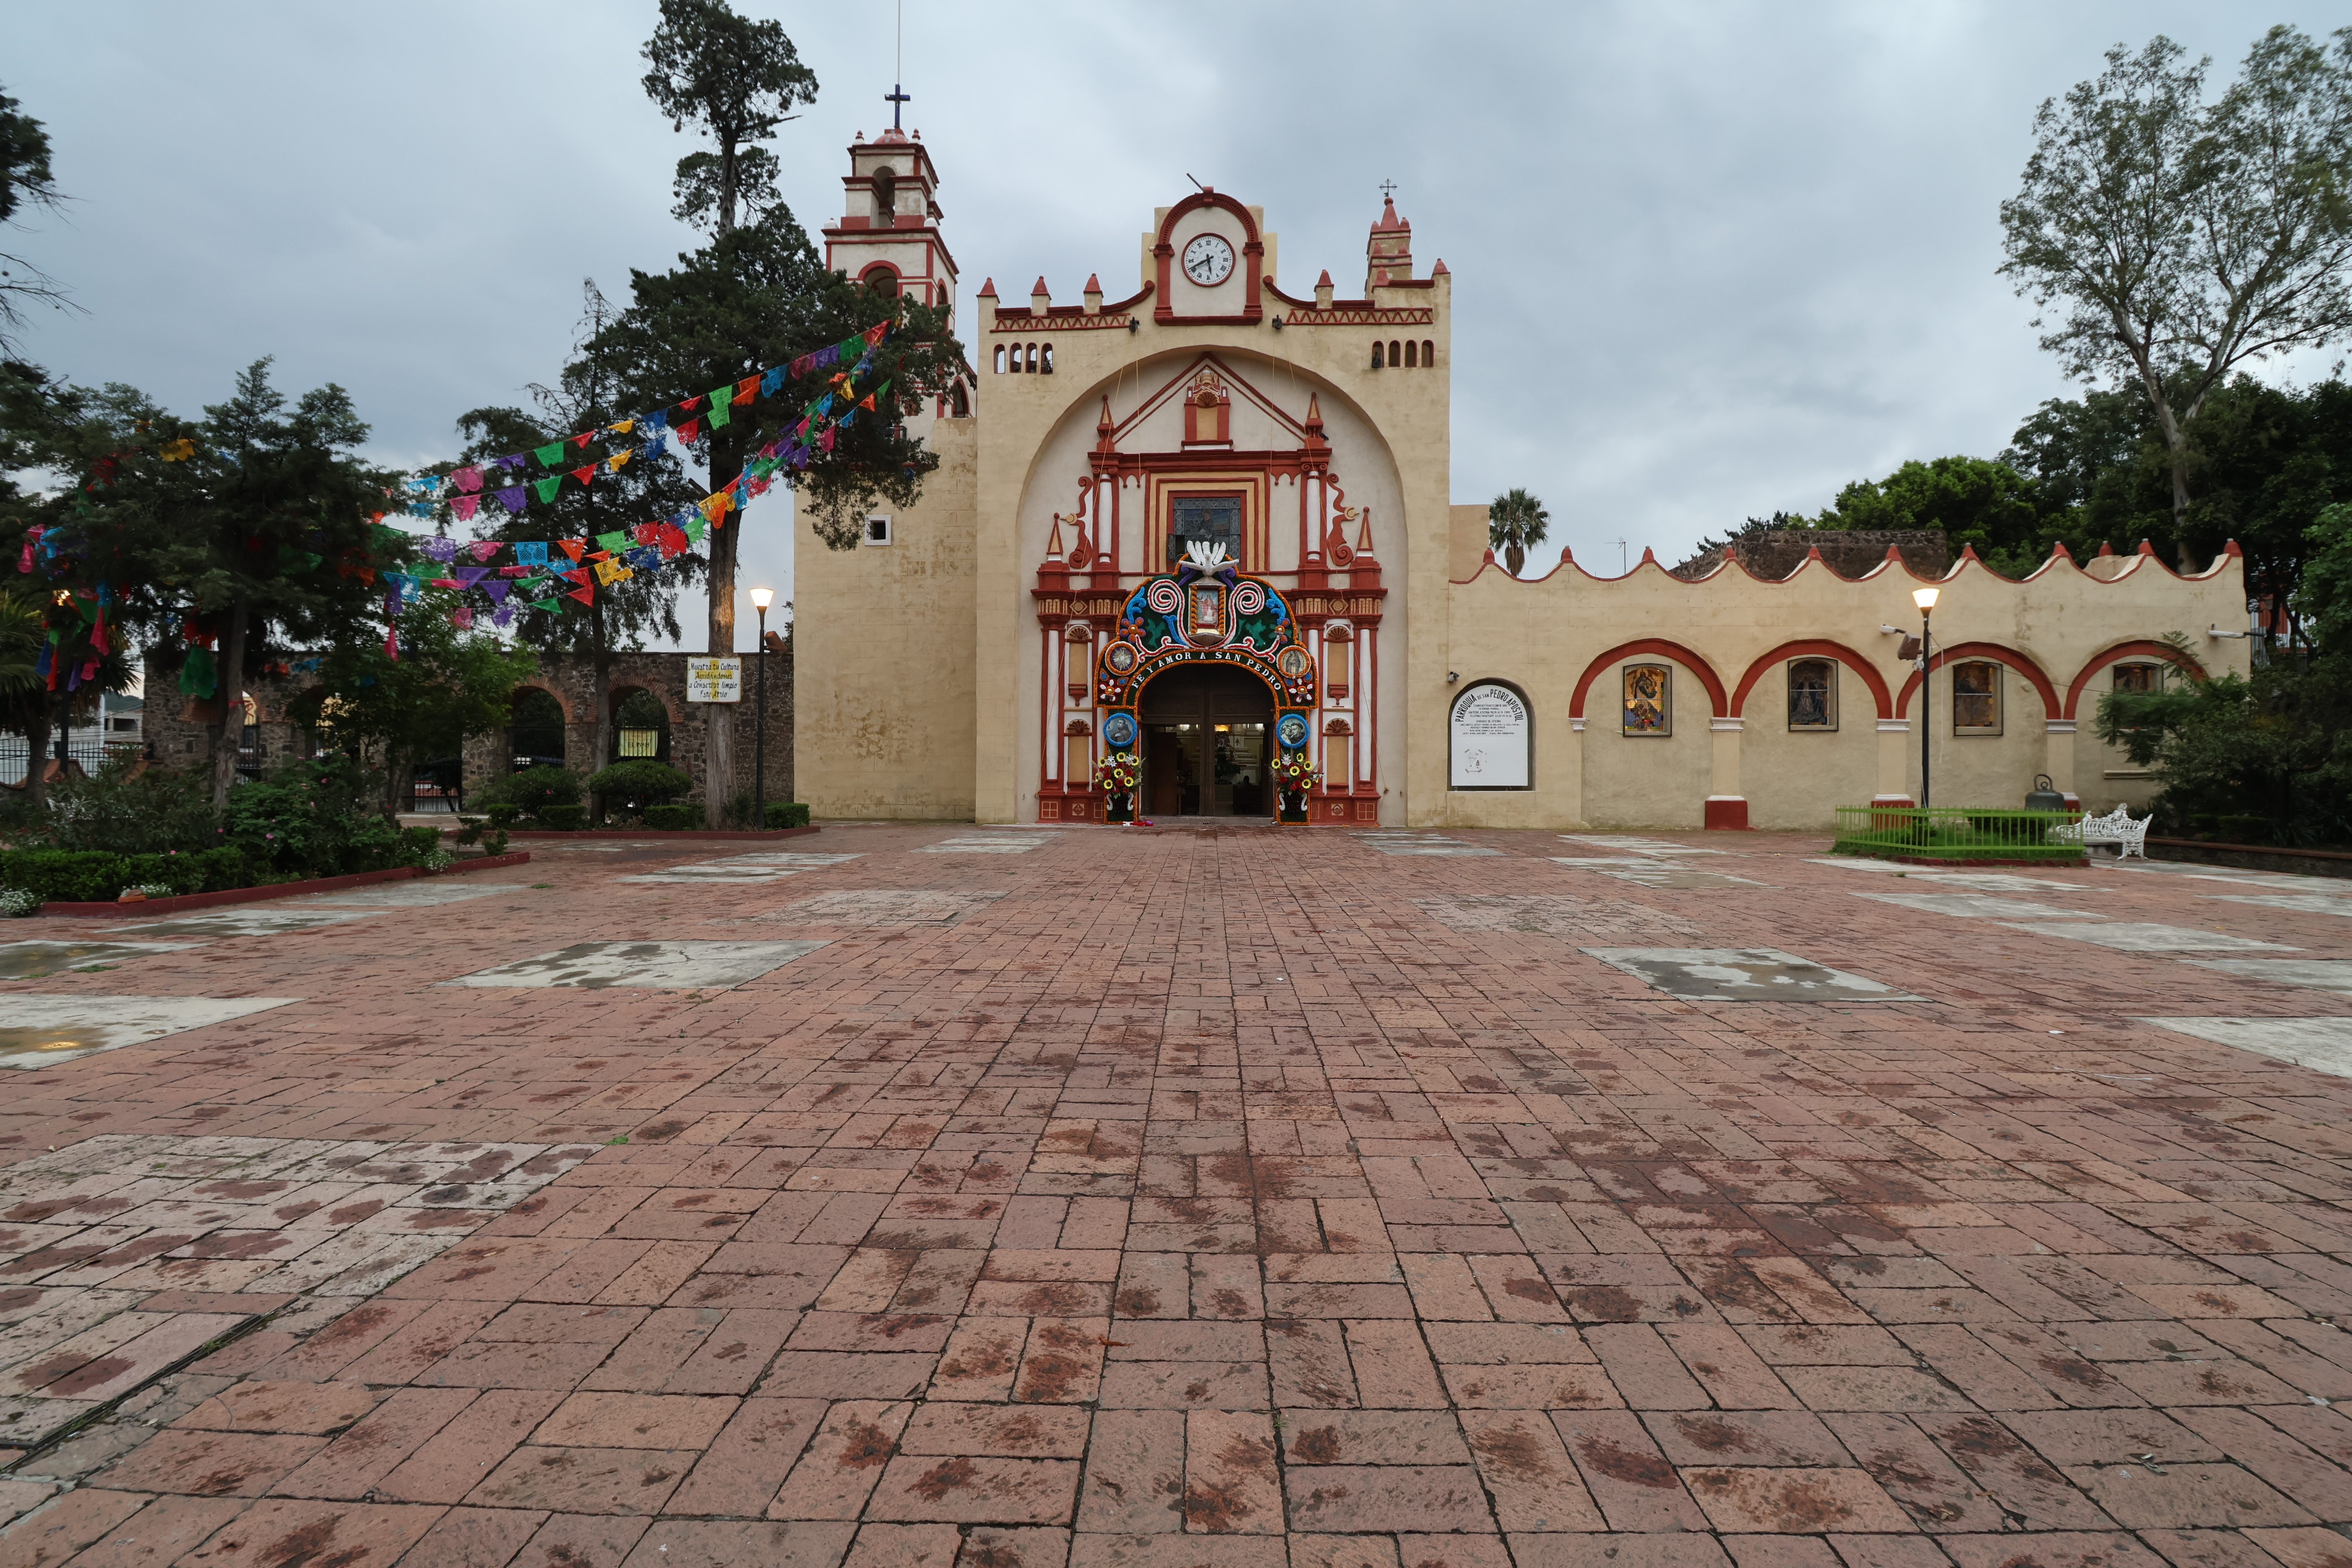
\includegraphics[width=\textwidth,height=7.2cm,keepaspectratio=false]{img/FotosActuales/Parroquia/Parroquia1.JPEG}
        \caption{Vista general de la fachada principal y acceso atrial.}
        \label{subfig:parroquia-fachada}
    \end{subfigure}
    \hfill
    \begin{subfigure}[b]{0.48\textwidth}
        \centering
        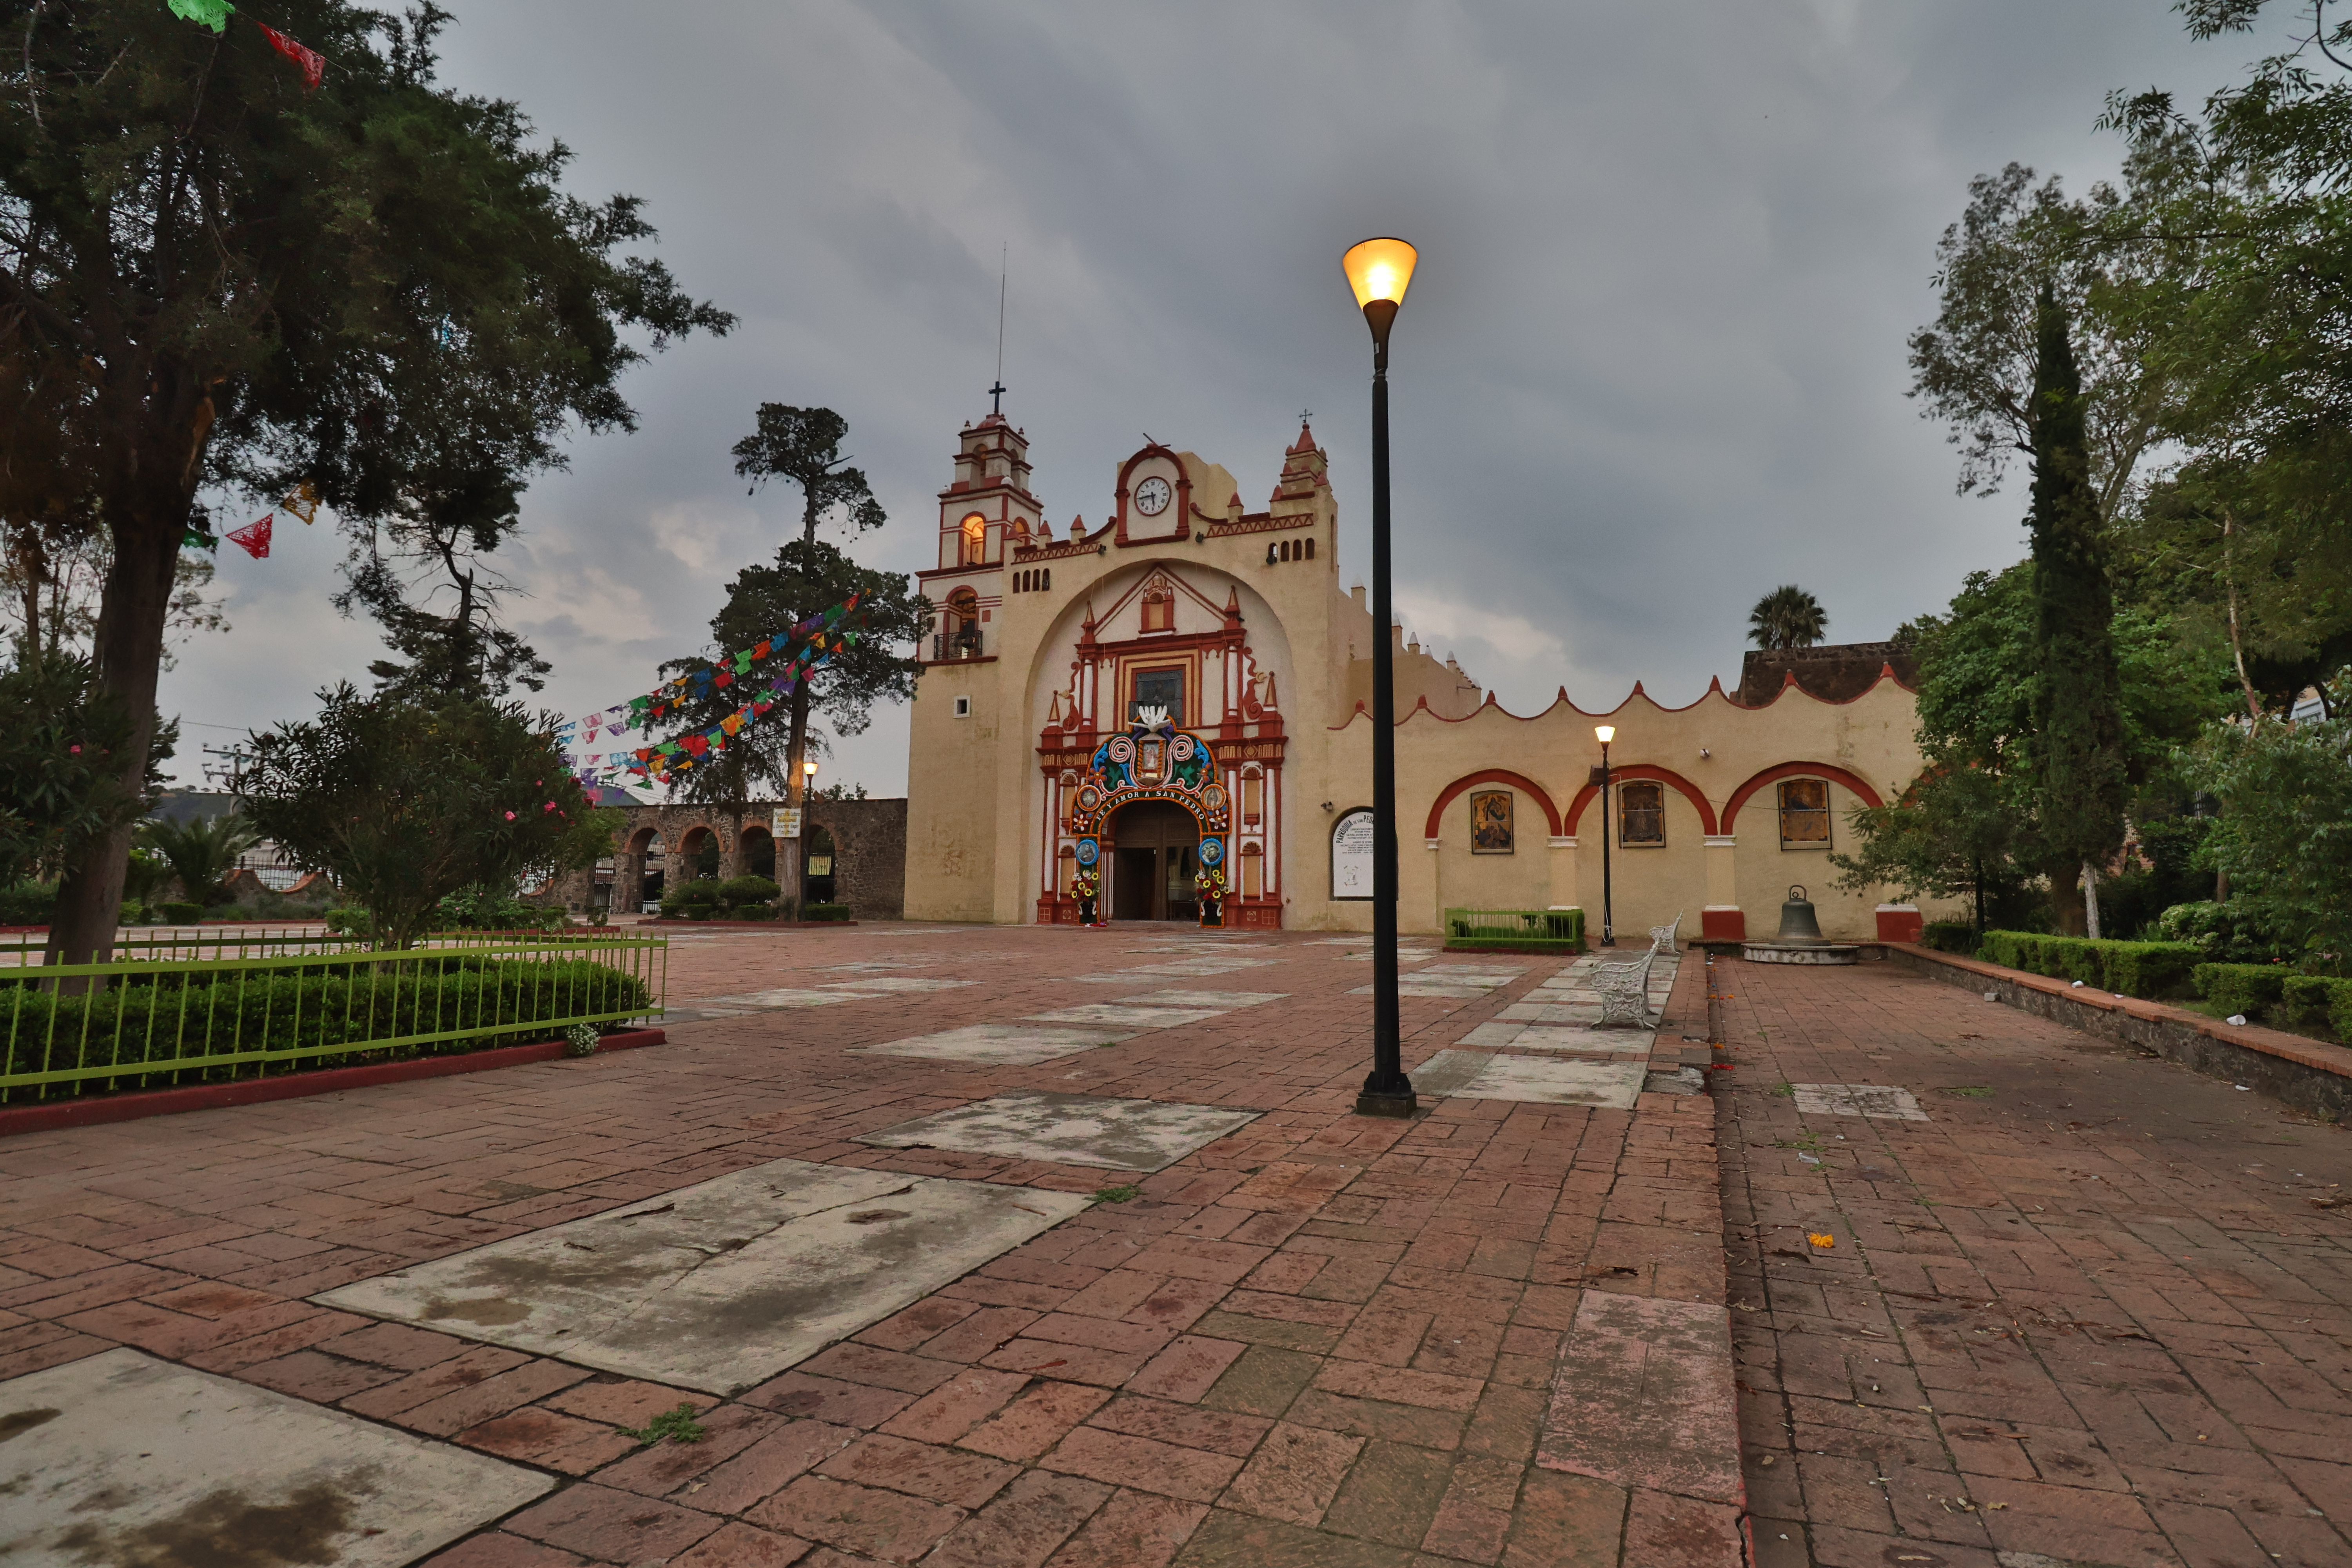
\includegraphics[width=\textwidth,height=7.2cm,keepaspectratio=false]{img/FotosActuales/Parroquia/Parroquia2.JPEG}
        \caption{Perspectiva lateral del cuerpo de la nave y contrafuertes.}
        \label{subfig:parroquia-lateral}
    \end{subfigure}
    
    \vspace{0.5cm} % Espaciado vertical controlado entre las filas de la cuadrícula
    
    % FILA 2: FOTOS INFERIORES (Lado a Lado)
    \begin{subfigure}[b]{0.48\textwidth}
        \centering
        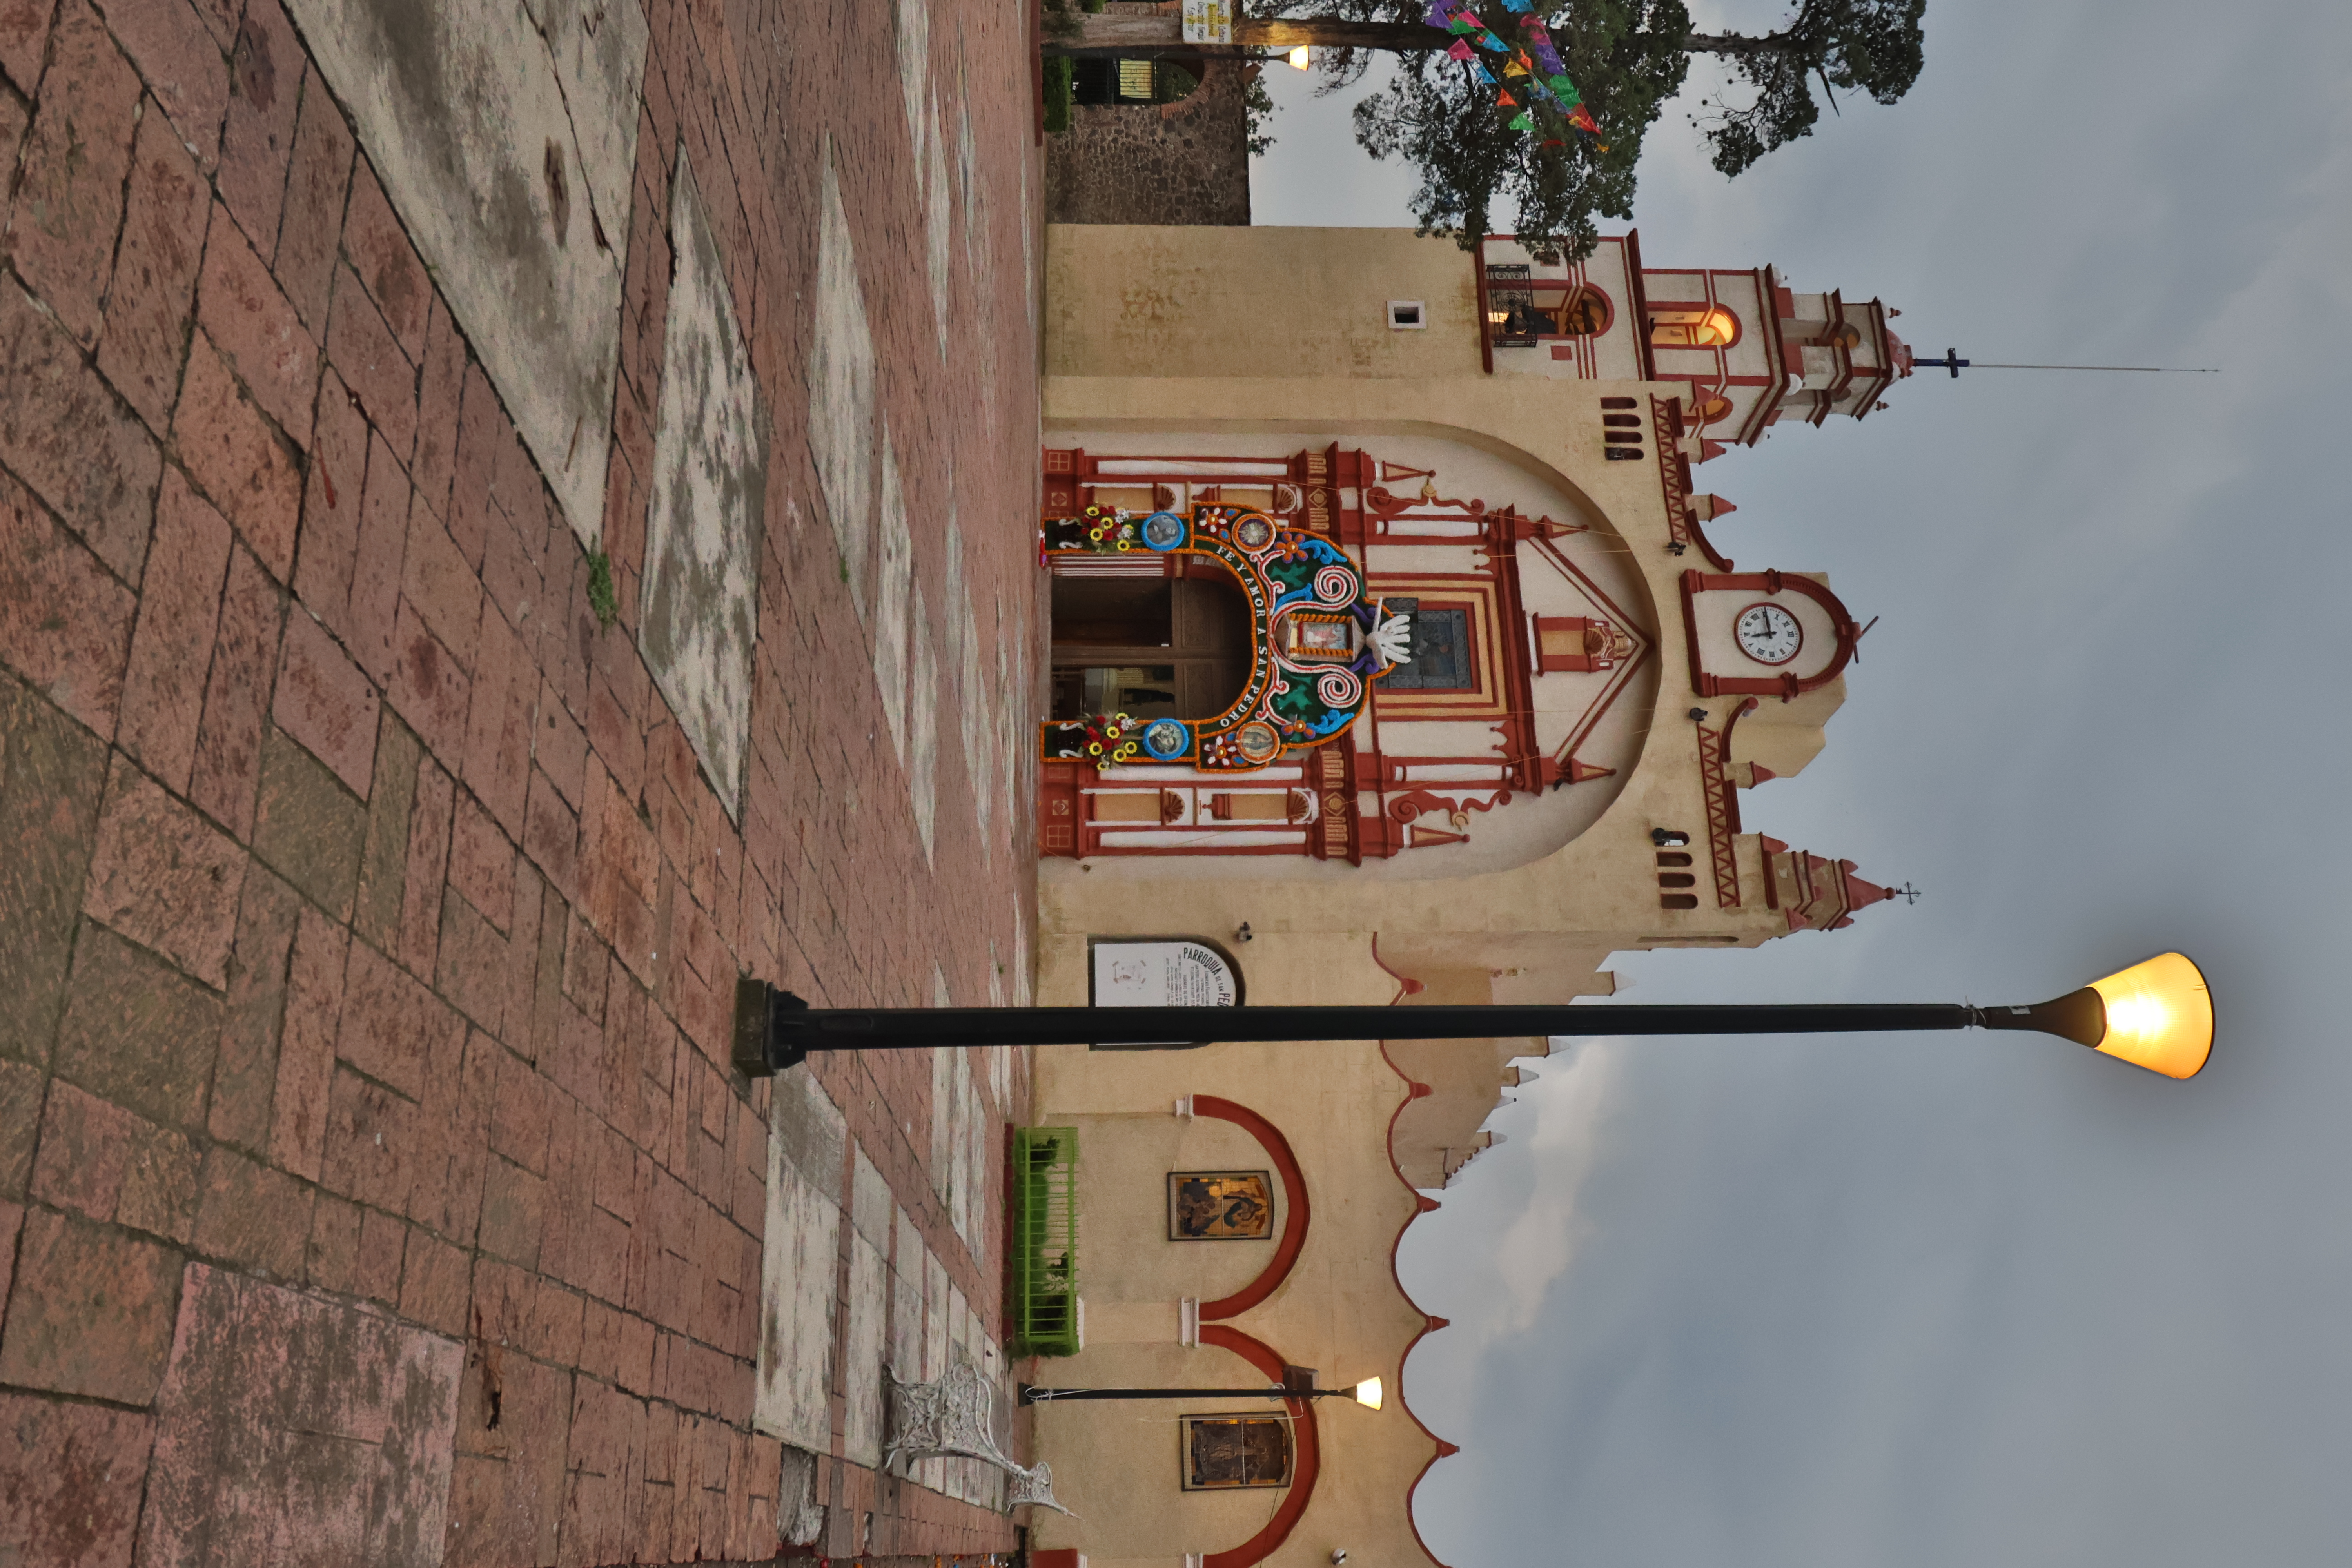
\includegraphics[width=\textwidth,height=7.2cm,keepaspectratio=false]{img/FotosActuales/Parroquia/Parroquia3.JPEG}
        \caption{Detalle de la torre del campanario y remates ornamentales.}
        \label{subfig:parroquia-torre}
    \end{subfigure}
    \hfill
    \begin{subfigure}[b]{0.48\textwidth}
        \centering
        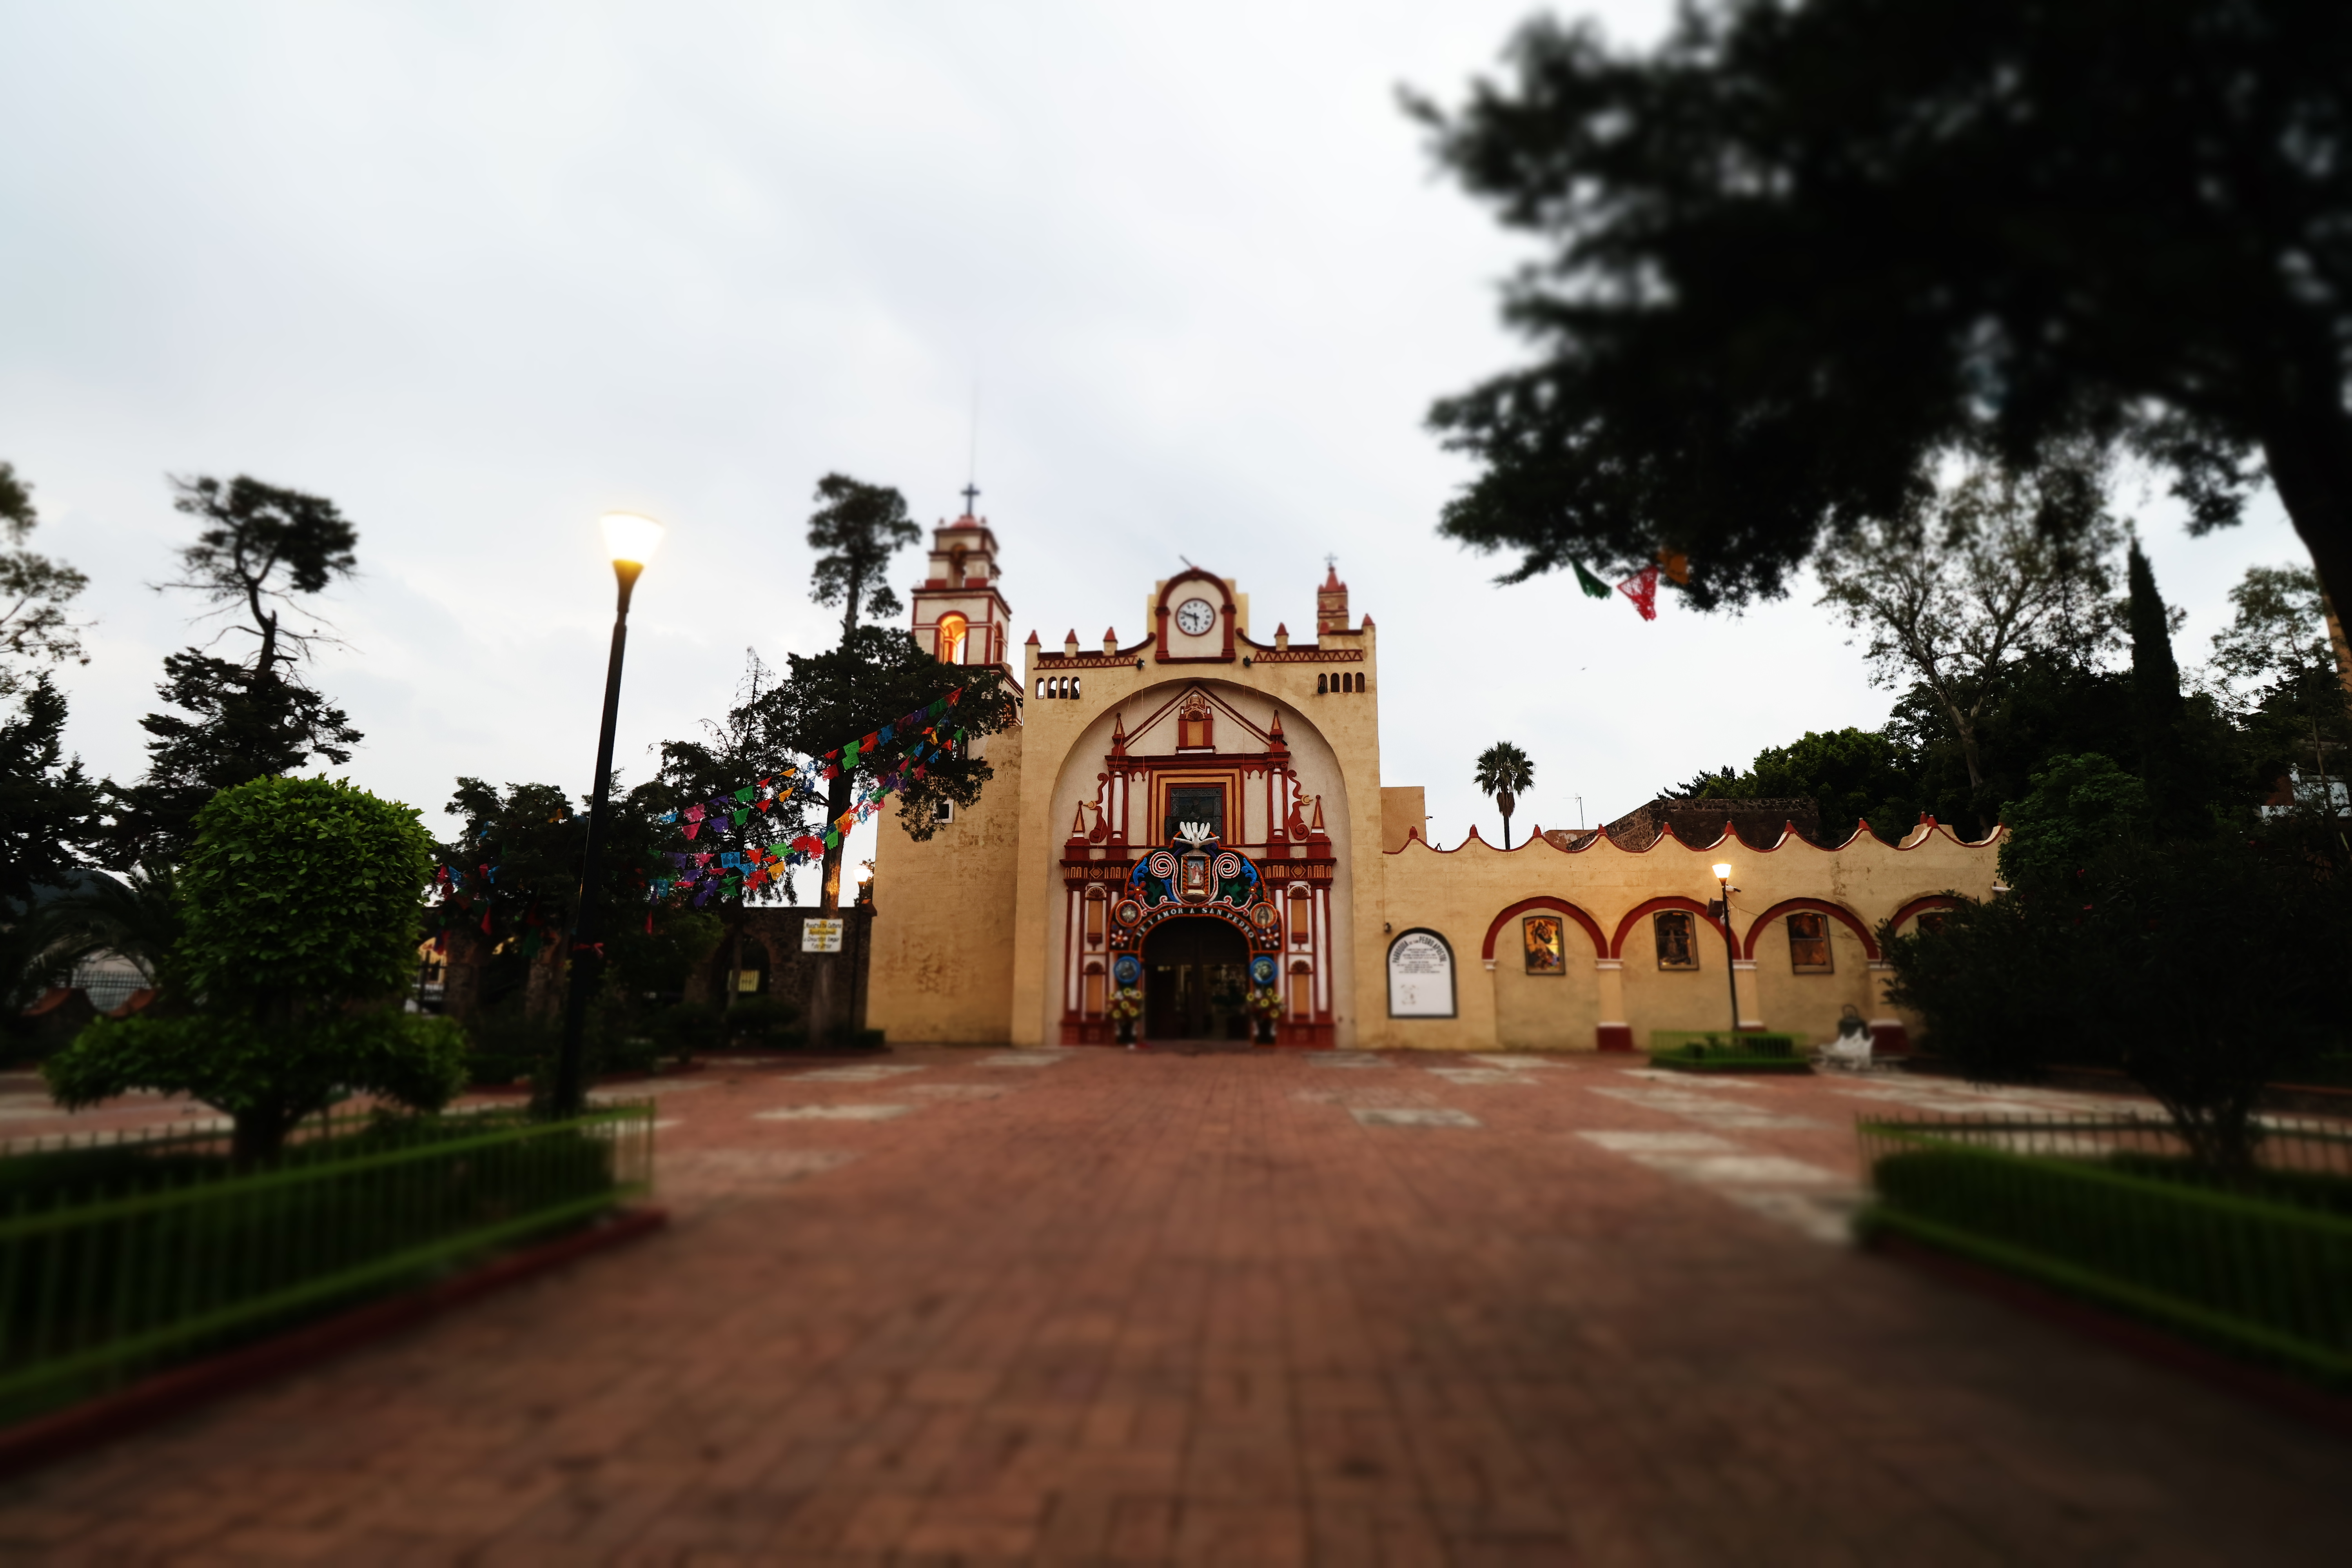
\includegraphics[width=\textwidth,height=7.2cm,keepaspectratio=false]{img/FotosActuales/Parroquia/Parroquia4.JPEG}
        \caption{Entorno inmediato urbano y articulación con la plaza.}
        \label{subfig:parroquia-entorno}
    \end{subfigure}
    
    \vspace{0.4cm}
    % Pie de figura maestro con metadatos técnicos exigidos en tesis y planes maestros
    \caption{Cuadrícula de diagnóstico cartográfico e iconográfico de la Parroquia de San 
    Pedro Apóstol. \textbf{ID de Catálogo:} INAH-DF-MilpaAlta-001. \textbf{Época:} 
    Siglo XVI (Fundación oficial: 1532). \textbf{Ubicación:} Traza Central, 
    San Pedro Atocpan. \textbf{Fuente y Autoría:} Fotografía de campo, obra 
    original de la autoria del proyeccionista (Galigaribaldi).}
    \label{fig:cuadricula-parroquia}
\end{figure}
\newpage

% =========================================================================
% FICHA DE INVENTARIO PATRIMONIAL: CAPILLA DE SAN MARTÍN CABALLERO
% =========================================================================
\newpage
\section{Fichas de Inventario: Capilla de San Martín Caballero (Yencuictlalpan)}
\label{anexo:ficha-capilla}

Este apartado documenta visualmente el estado general y los procesos de intervención 
contemporánea del recinto histórico de Yencuictlalpan, identificado en el análisis de 
riesgo como el epicentro de la memoria colectiva y de refugio tras el desastre hídrico de 1935.

\begin{figure}[p]
    \centering
    \caption*{--- FICHA DE REGISTRO PATRIMONIAL INMUEBLE: CAPILLA DE SAN MARTÍN ---}
    \vspace{0.3cm}
    
    % FILA 1: FOTO PRINCIPAL (Ancho completo)
    \begin{subfigure}[b]{\textwidth}
        \centering
        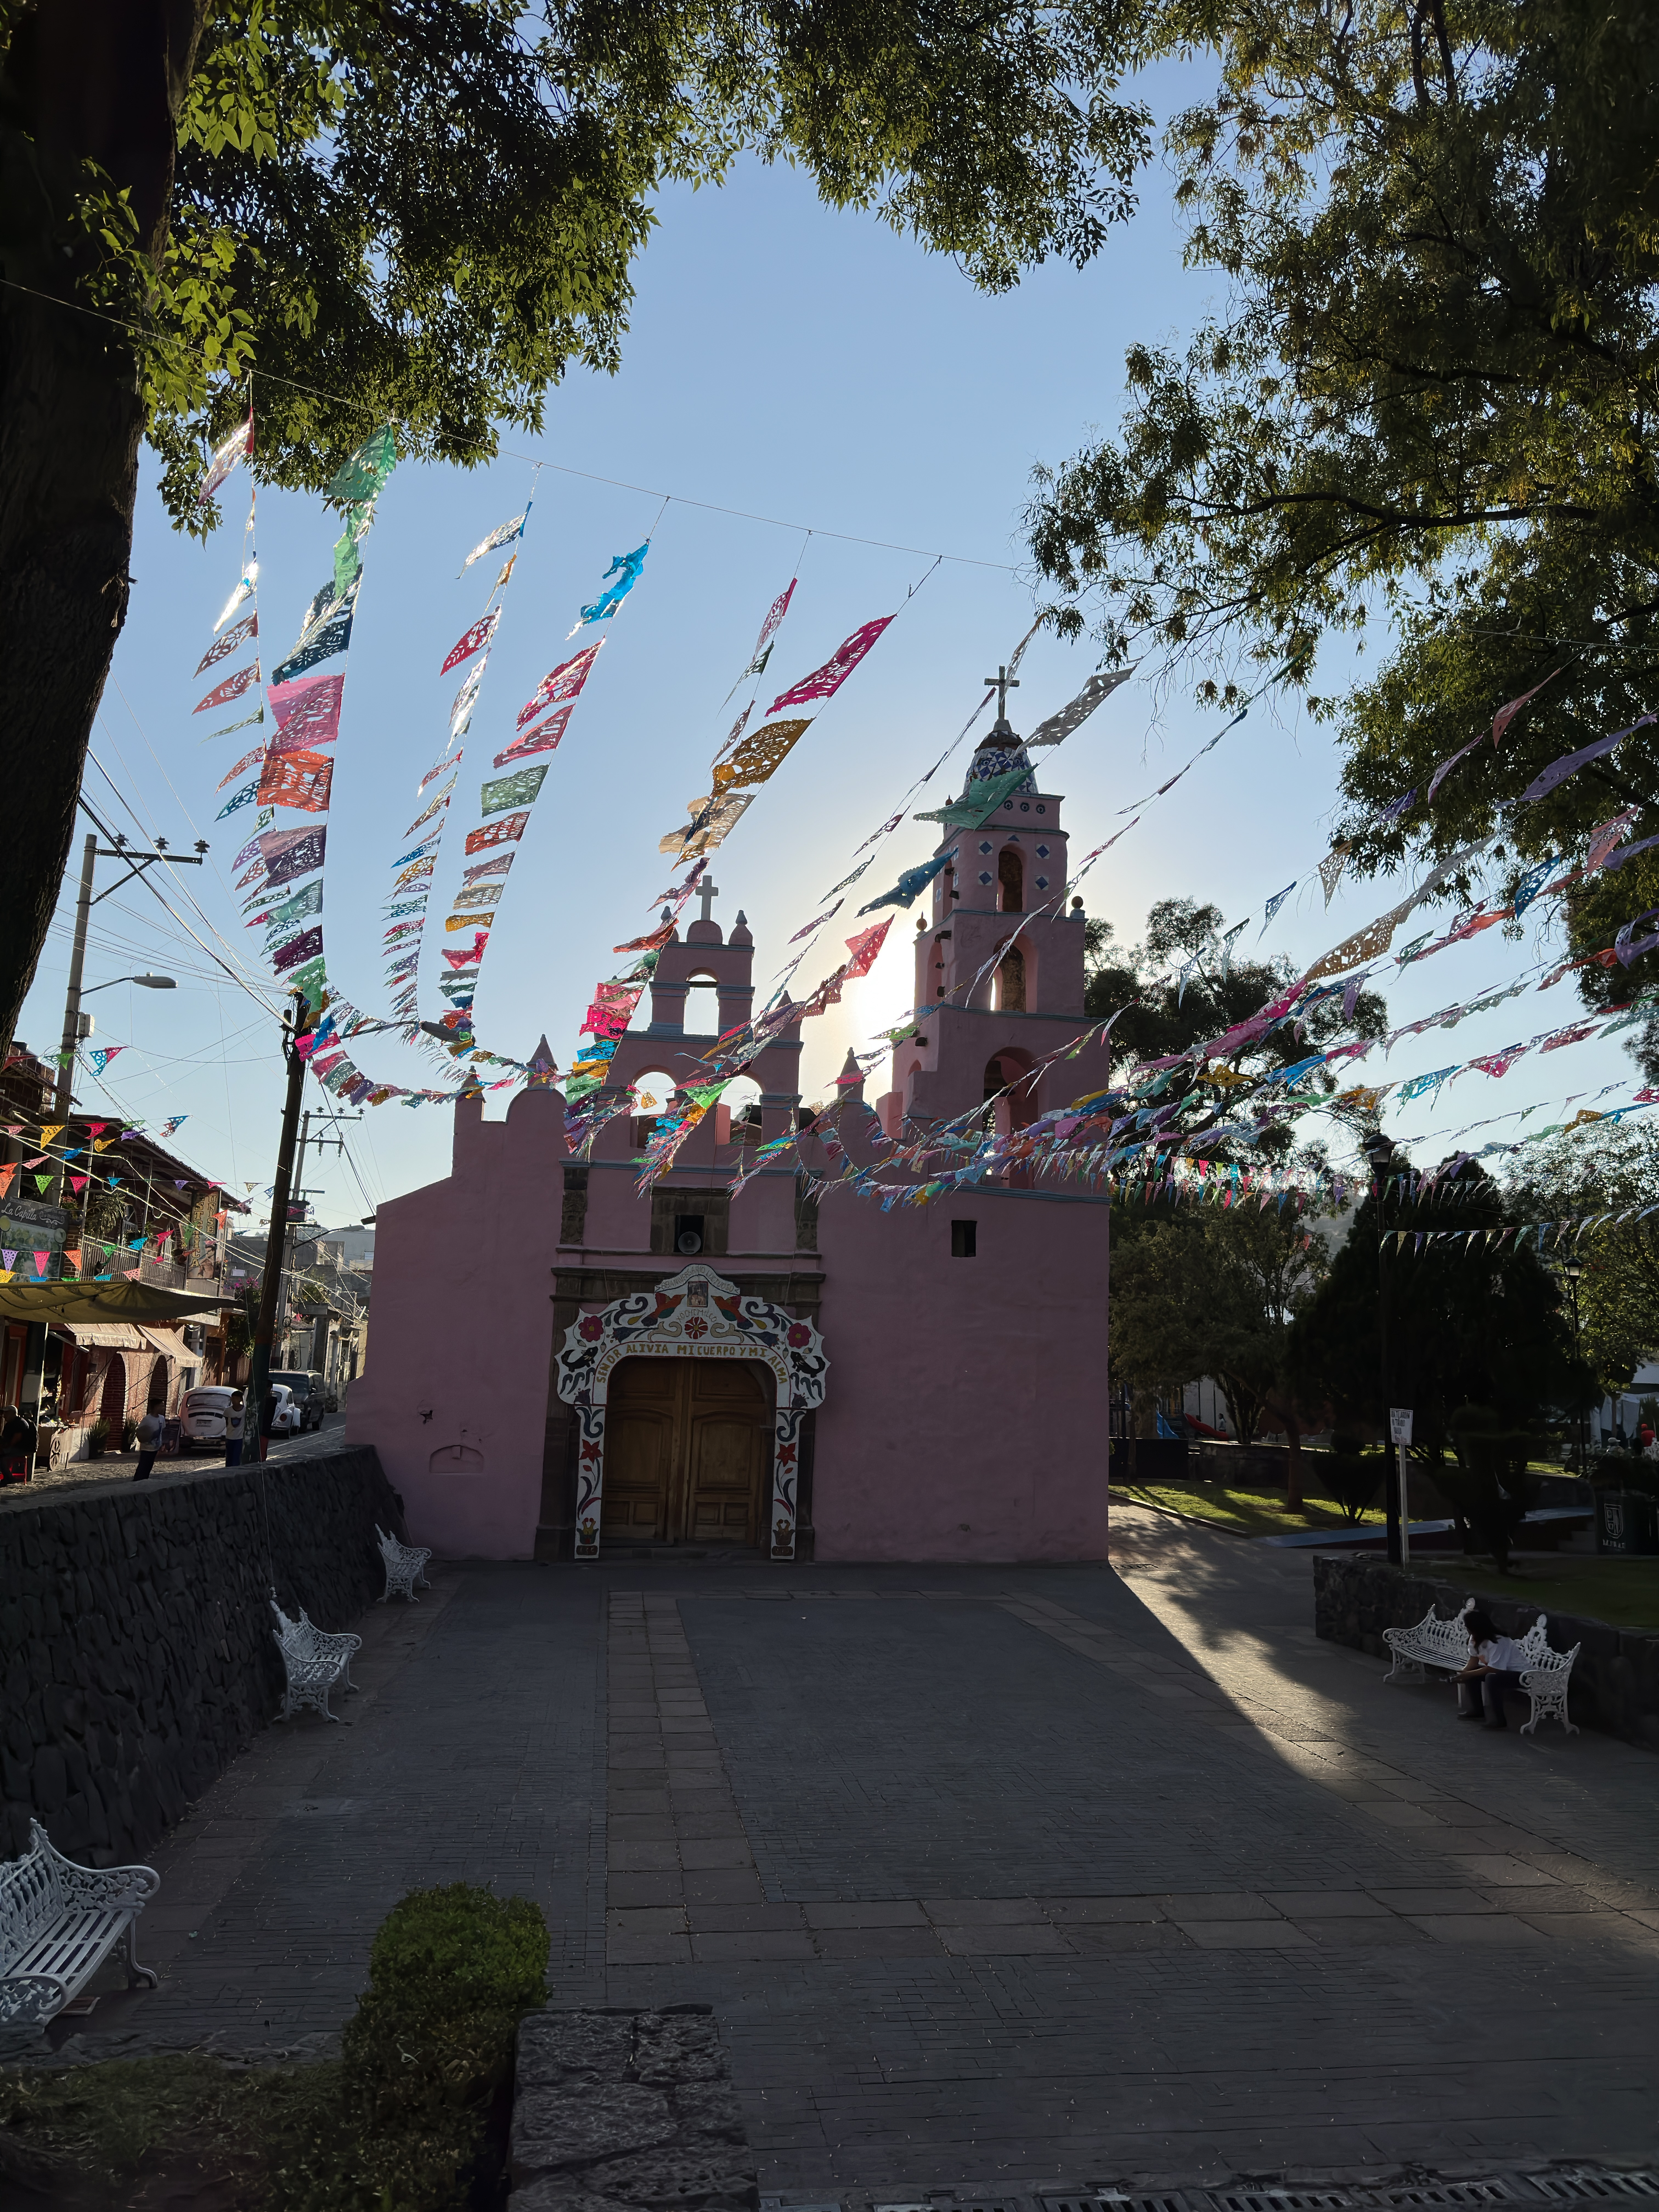
\includegraphics[width=\textwidth,height=9cm,keepaspectratio=false]{img/FotosActuales/CapillaSanMartin/CapillaColorOriginal.JPEG}
        \caption{Vista general de la Capilla de San Martín (Yencuictlalpan), mostrando la cromática y proporción de la fachada.}
        \label{subfig:capilla-original}
    \end{subfigure}
    
    \vspace{0.5cm} % Espaciado vertical entre la imagen principal y los detalles
    
    % FILA 2: FOTOS DE REMODELACIÓN (Lado a Lado)
    \begin{subfigure}[b]{0.48\textwidth}
        \centering
        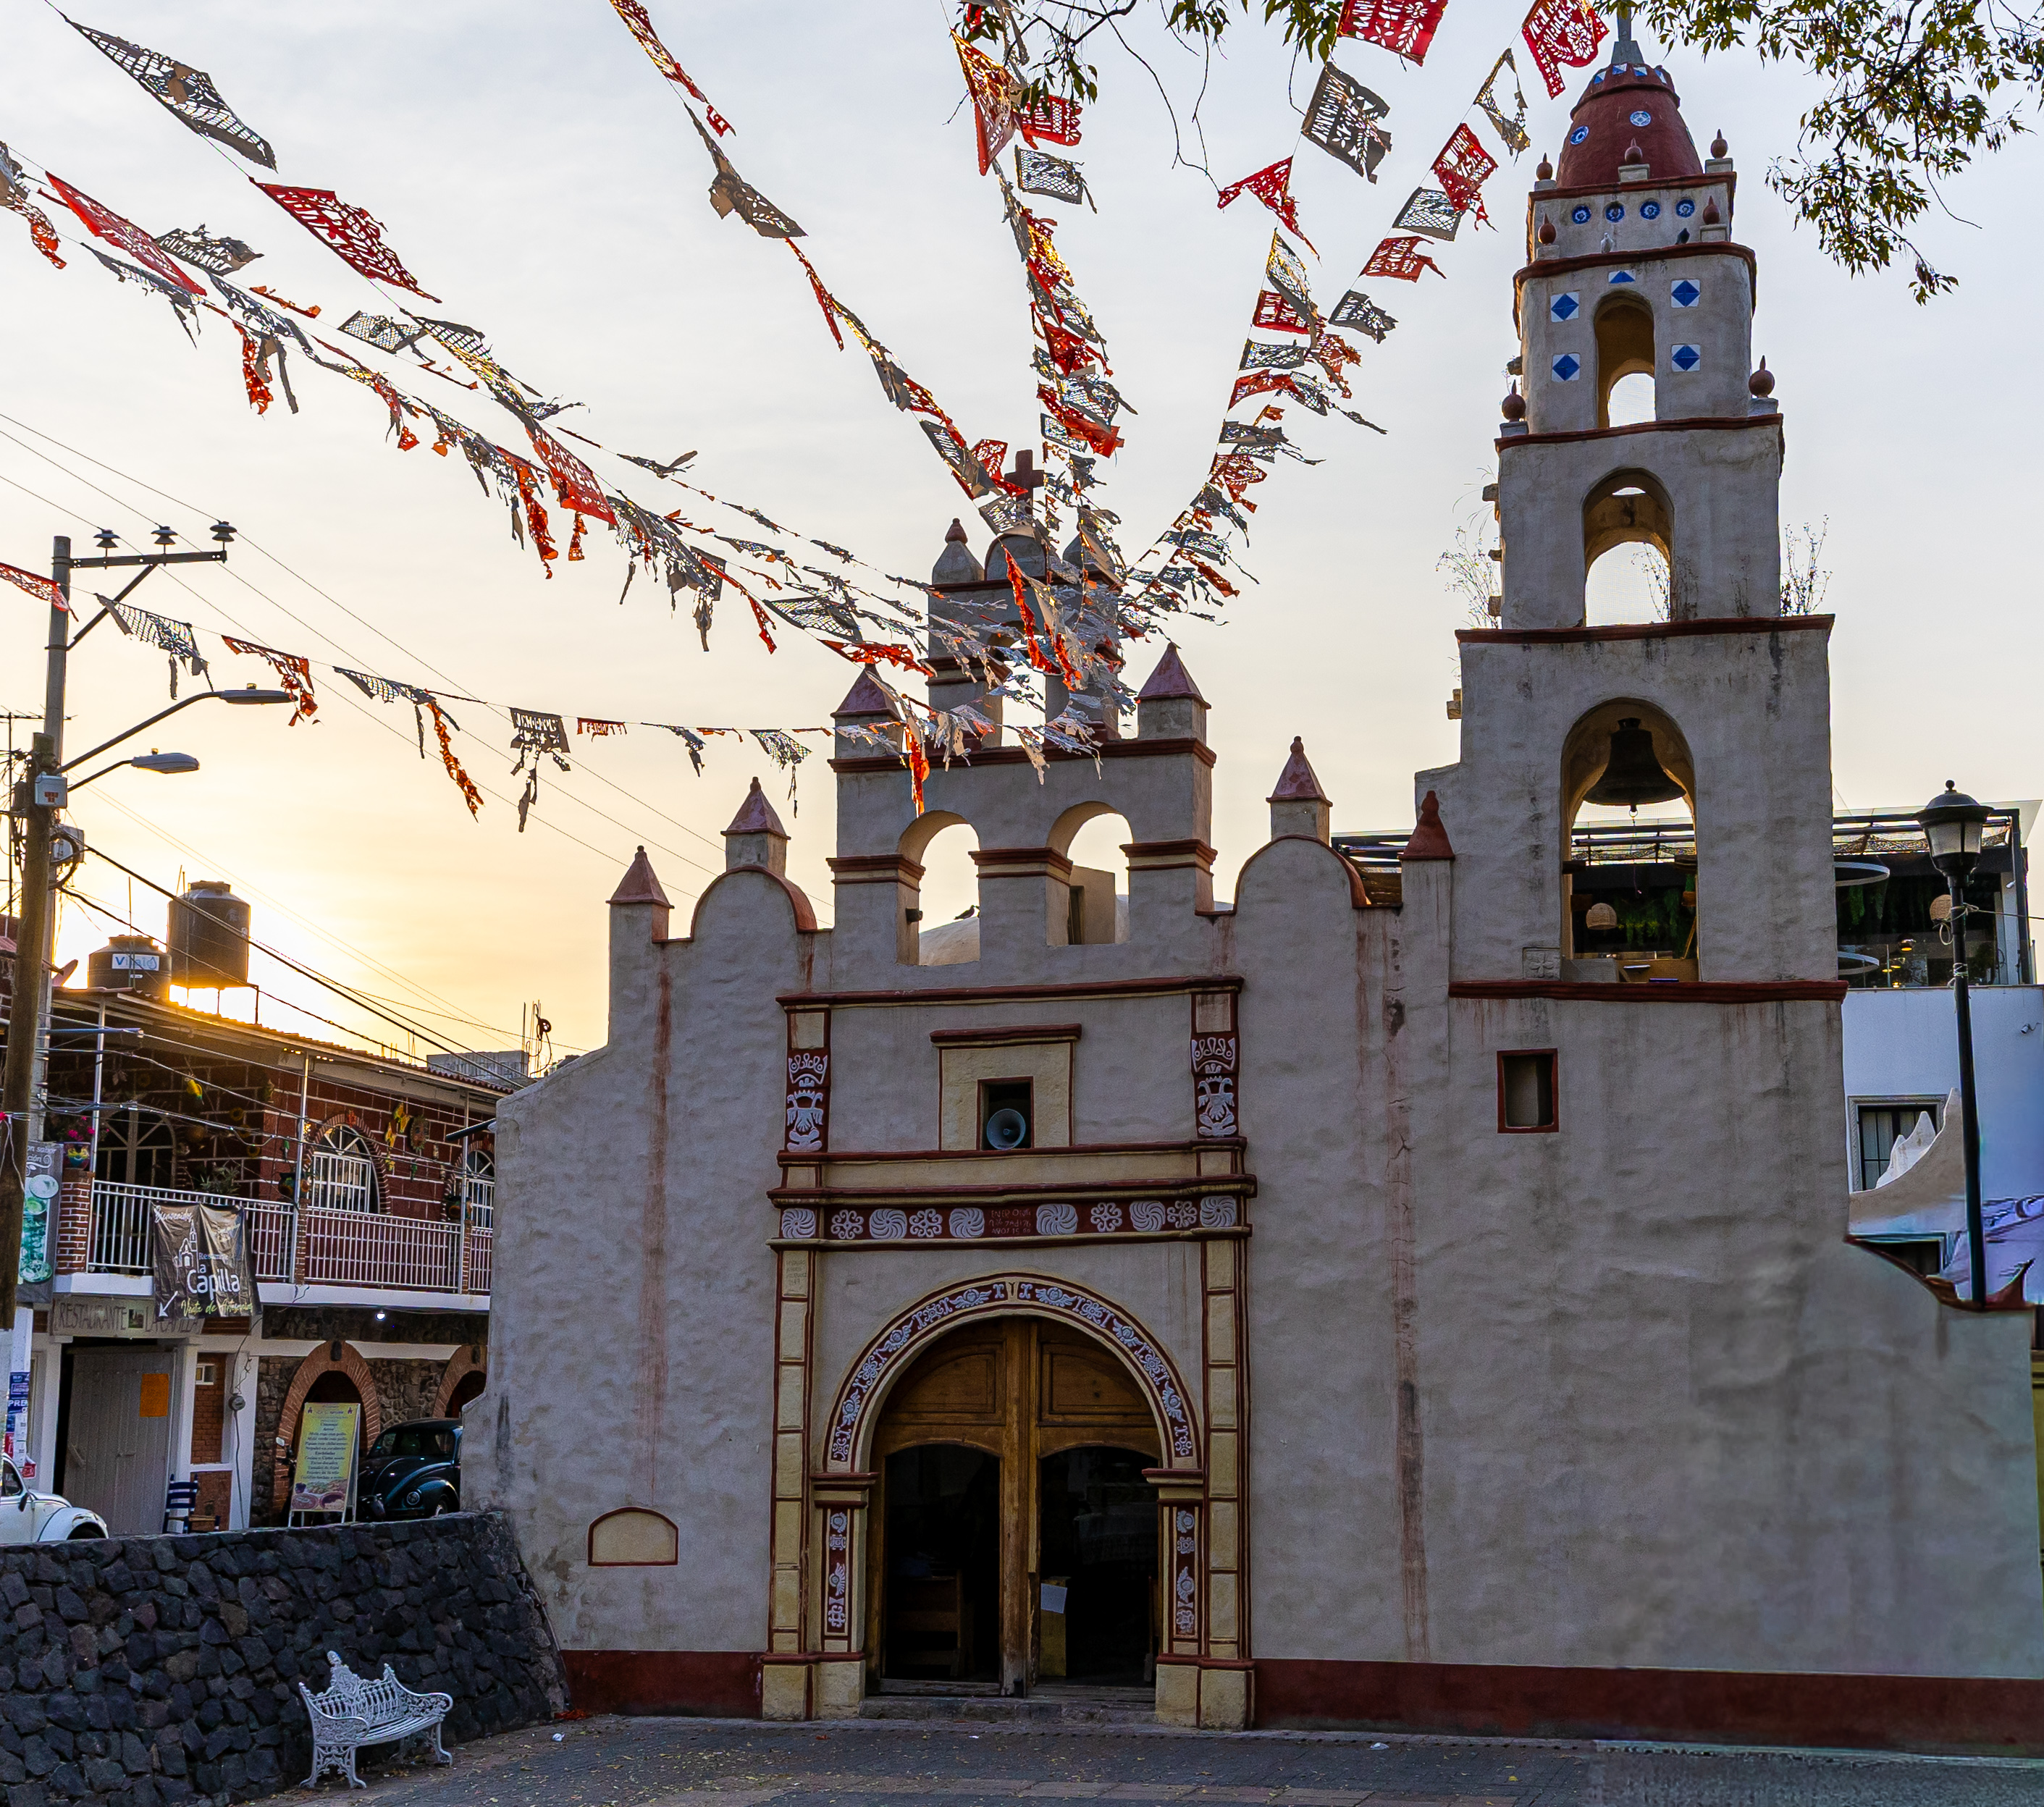
\includegraphics[width=\textwidth,height=7cm,keepaspectratio=false]{img/FotosActuales/CapillaSanMartin/CapillaRemodelacion.JPEG}
        \caption{Detalle arquitectónico durante el proceso de intervención y consolidación física.}
        \label{subfig:capilla-remodelacion1}
    \end{subfigure}
    \hfill
    \begin{subfigure}[b]{0.48\textwidth}
        \centering
        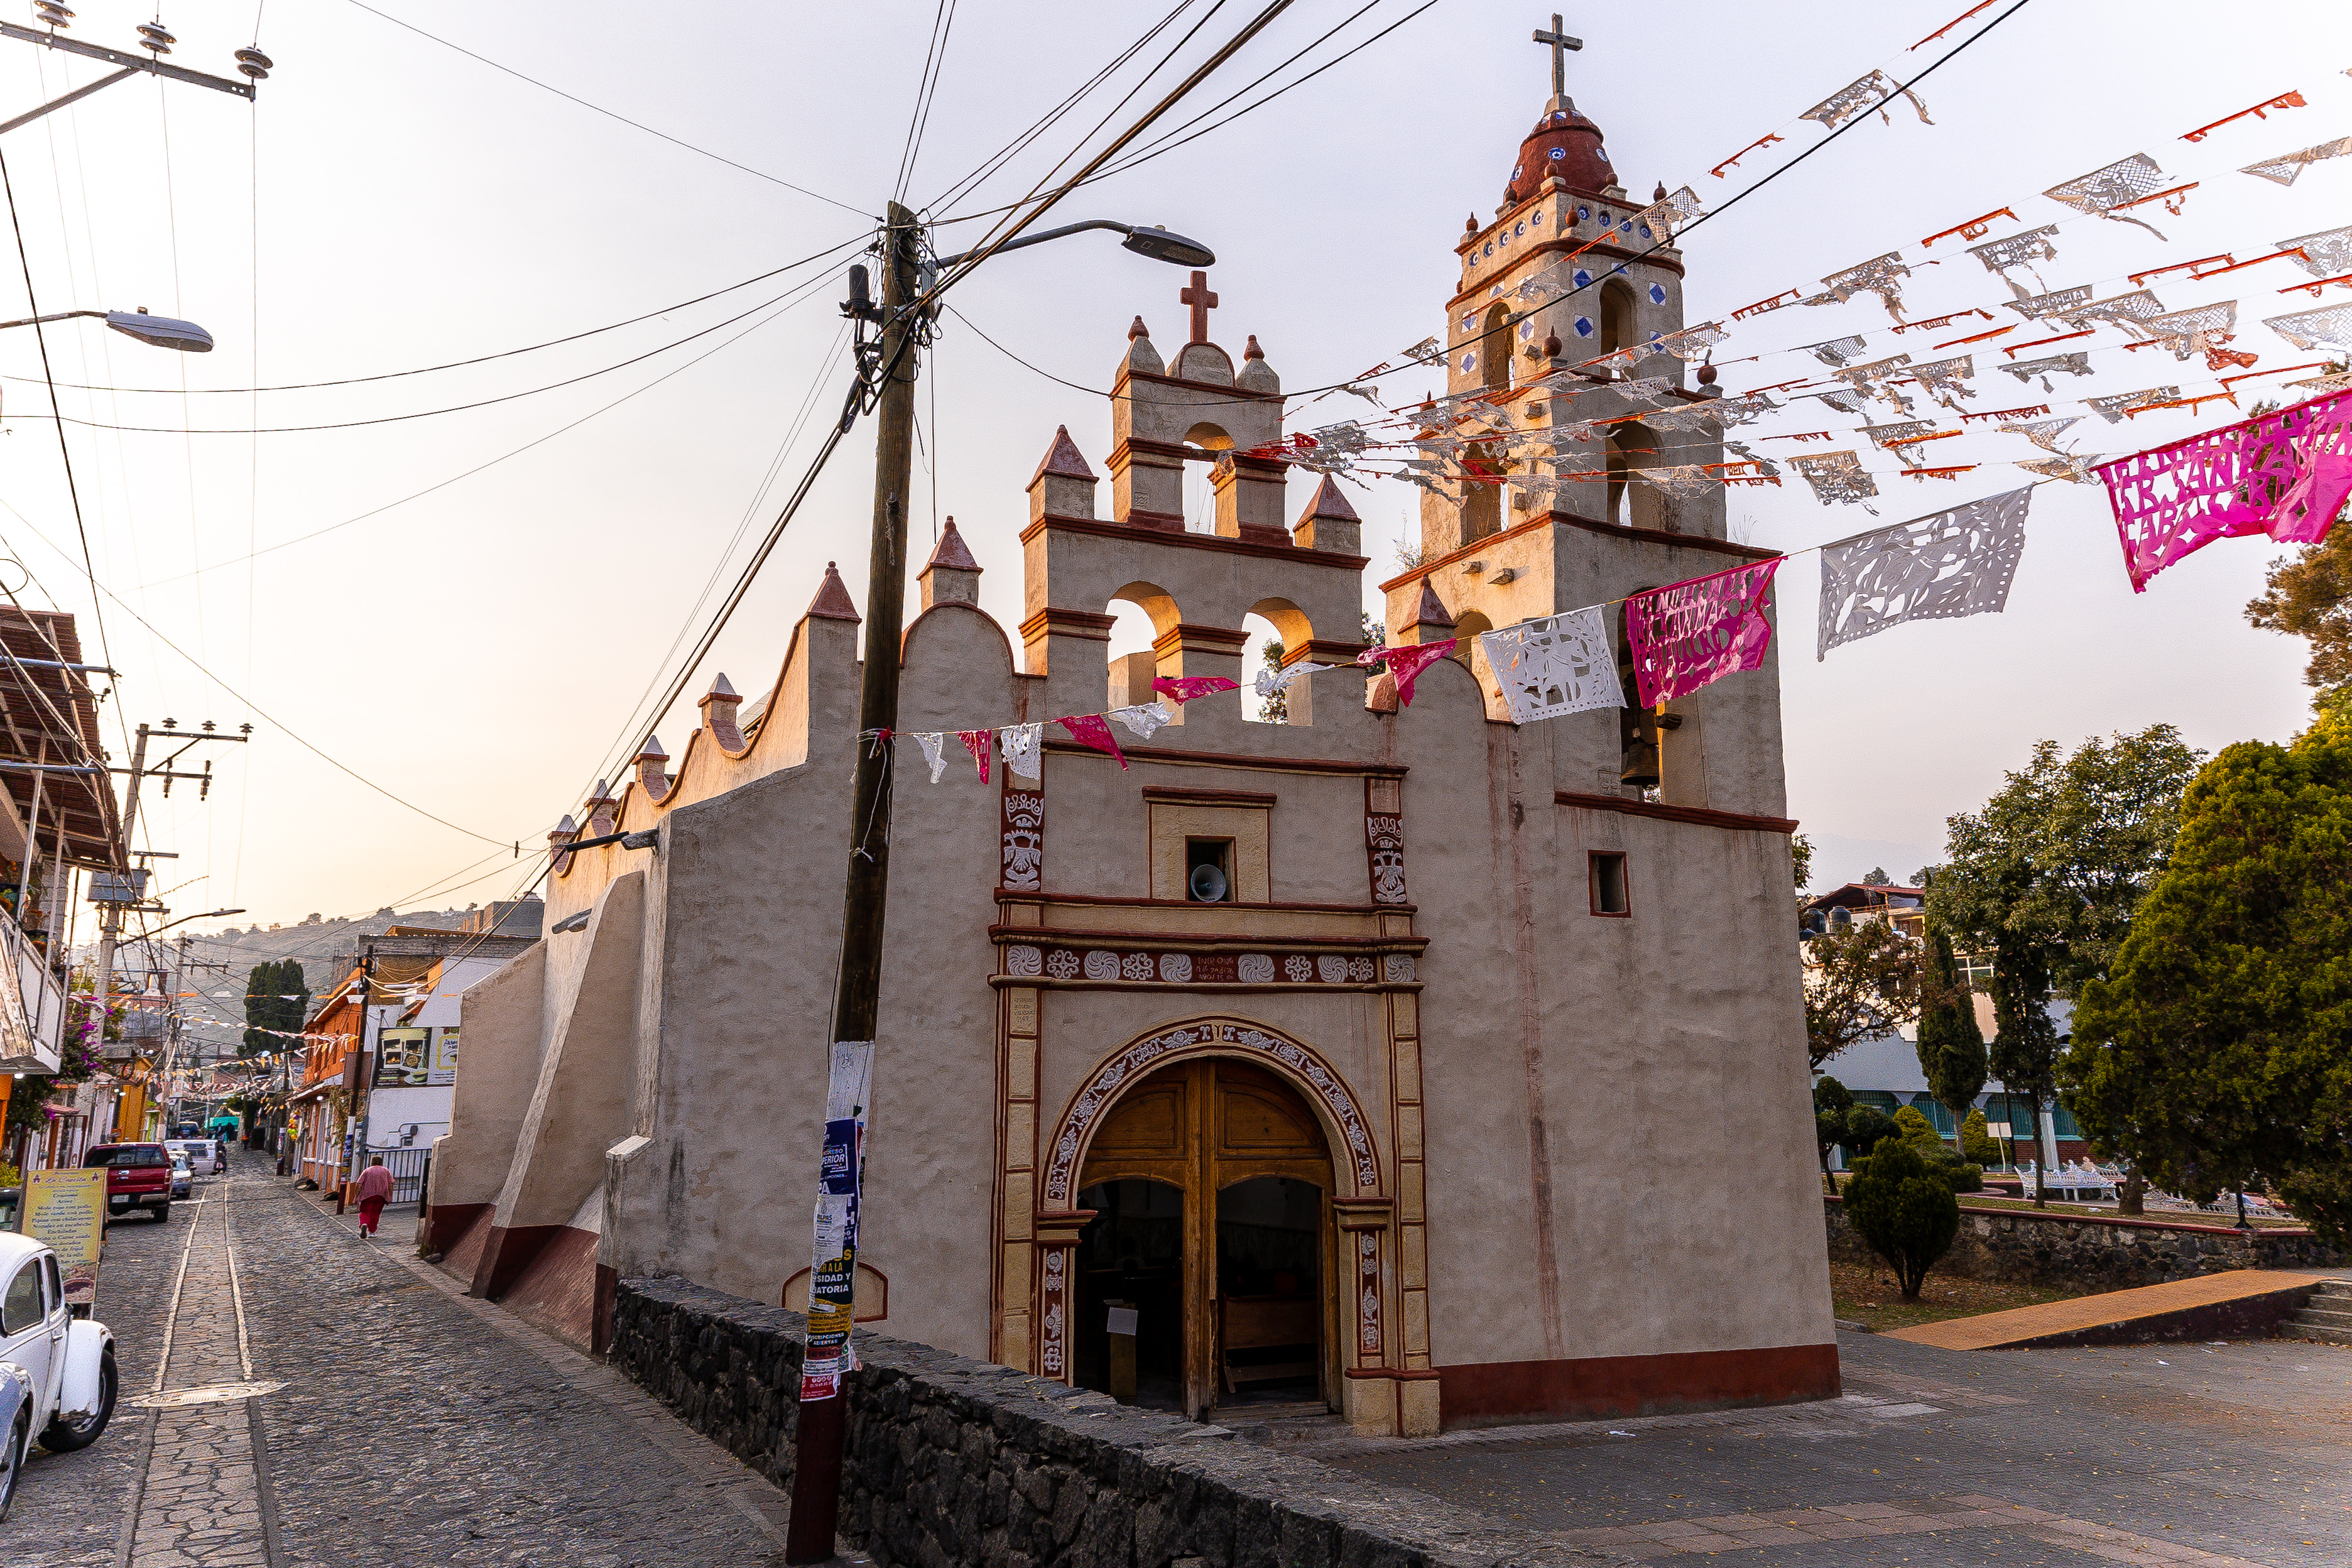
\includegraphics[width=\textwidth,height=7cm,keepaspectratio=false]{img/FotosActuales/CapillaSanMartin/CapillaRemodelacion2.JPEG}
        \caption{Avance estructural e integración de nuevos recubrimientos en el contexto histórico.}
        \label{subfig:capilla-remodelacion2}
    \end{subfigure}
    
    \vspace{0.4cm}
    % Pie de figura maestro con metadatos técnicos
    \caption{Registro fotográfico y proceso de intervención arquitectónica de la Capilla de San Martín Caballero. \textbf{ID de Catálogo:} 
    INAH-DF-MilpaAlta-002. \textbf{Relevancia:} Sitio histórico de resguardo durante la inundación de 1935. 
    \textbf{Ubicación:} Polígono 2, San Pedro Atocpan. 
    \textbf{Fuente y Autoría:} Fotografía de campo, obra original de la autoria del proyeccionista (Galigaribaldi).}
    \label{fig:cuadricula-capilla}
\end{figure}
\newpage

% =========================================================================
% FICHA DE INVENTARIO PATRIMONIAL: SANTUARIO DEL SEÑOR DE LAS MISERICORDIAS
% =========================================================================
\newpage
\section{Fichas de Inventario: Santuario del Señor de las Misericordias}
\label{anexo:ficha-santuario}

Esta ficha técnica compila el levantamiento fotográfico del Santuario Moderno. 
El análisis formal del inmueble permite entender la ruptura tipológica con la traza tradicional 
y la consolidación de nuevos hitos visuales a gran escala financiados por el tejido social local.

\begin{figure}[p] % 'p' destina la página completa exclusivamente para la cuadrícula fotográfica
    \centering
    \caption*{--- FICHA DE REGISTRO PATRIMONIAL INMUEBLE: SANTUARIO MODERNO ---}
    \vspace{0.3cm}
    
    % FILA 1: FOTOS SUPERIORES (Simbiosis geométrica y volumetría)
    \begin{subfigure}[b]{0.48\textwidth}
        \centering
        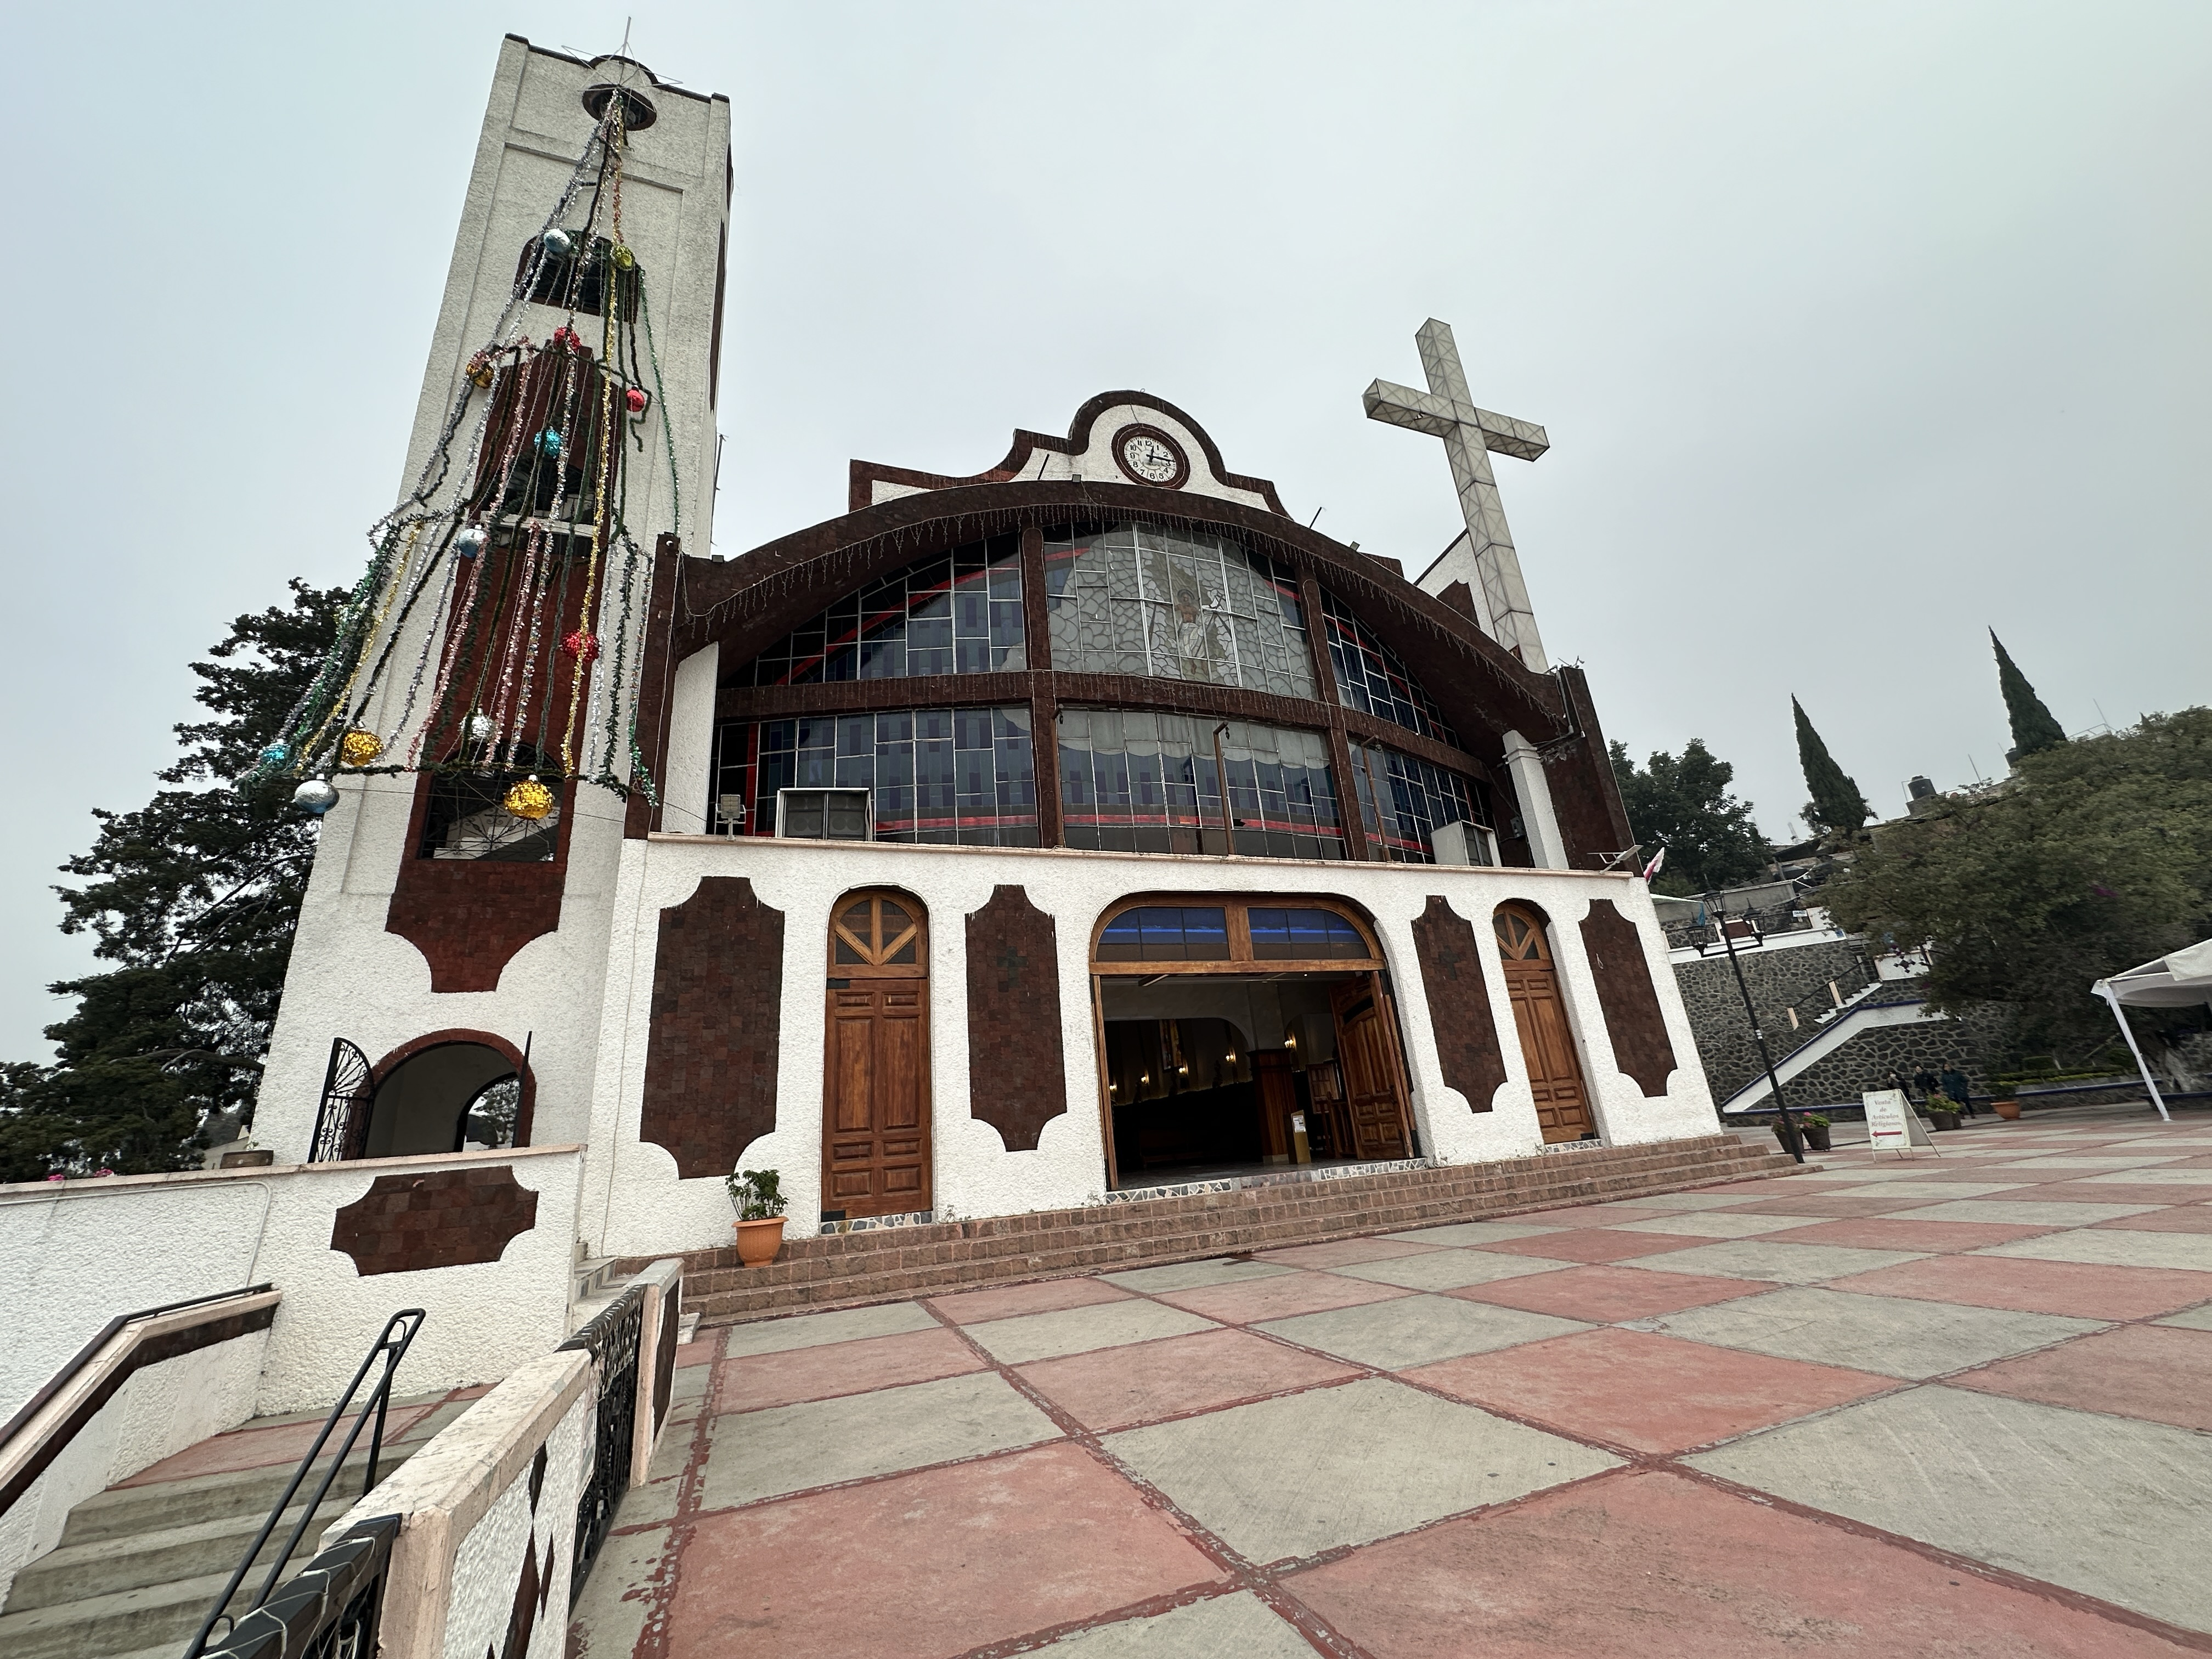
\includegraphics[width=\textwidth,height=7.2cm,keepaspectratio=false]{img/FotosActuales/TemploSrMisercordias/Tempo1.JPEG}
        \caption{Perspectiva de la fachada principal y geometría de la cubierta.}
        \label{subfig:santuario-fachada}
    \end{subfigure}
    \hfill
    \begin{subfigure}[b]{0.48\textwidth}
        \centering
        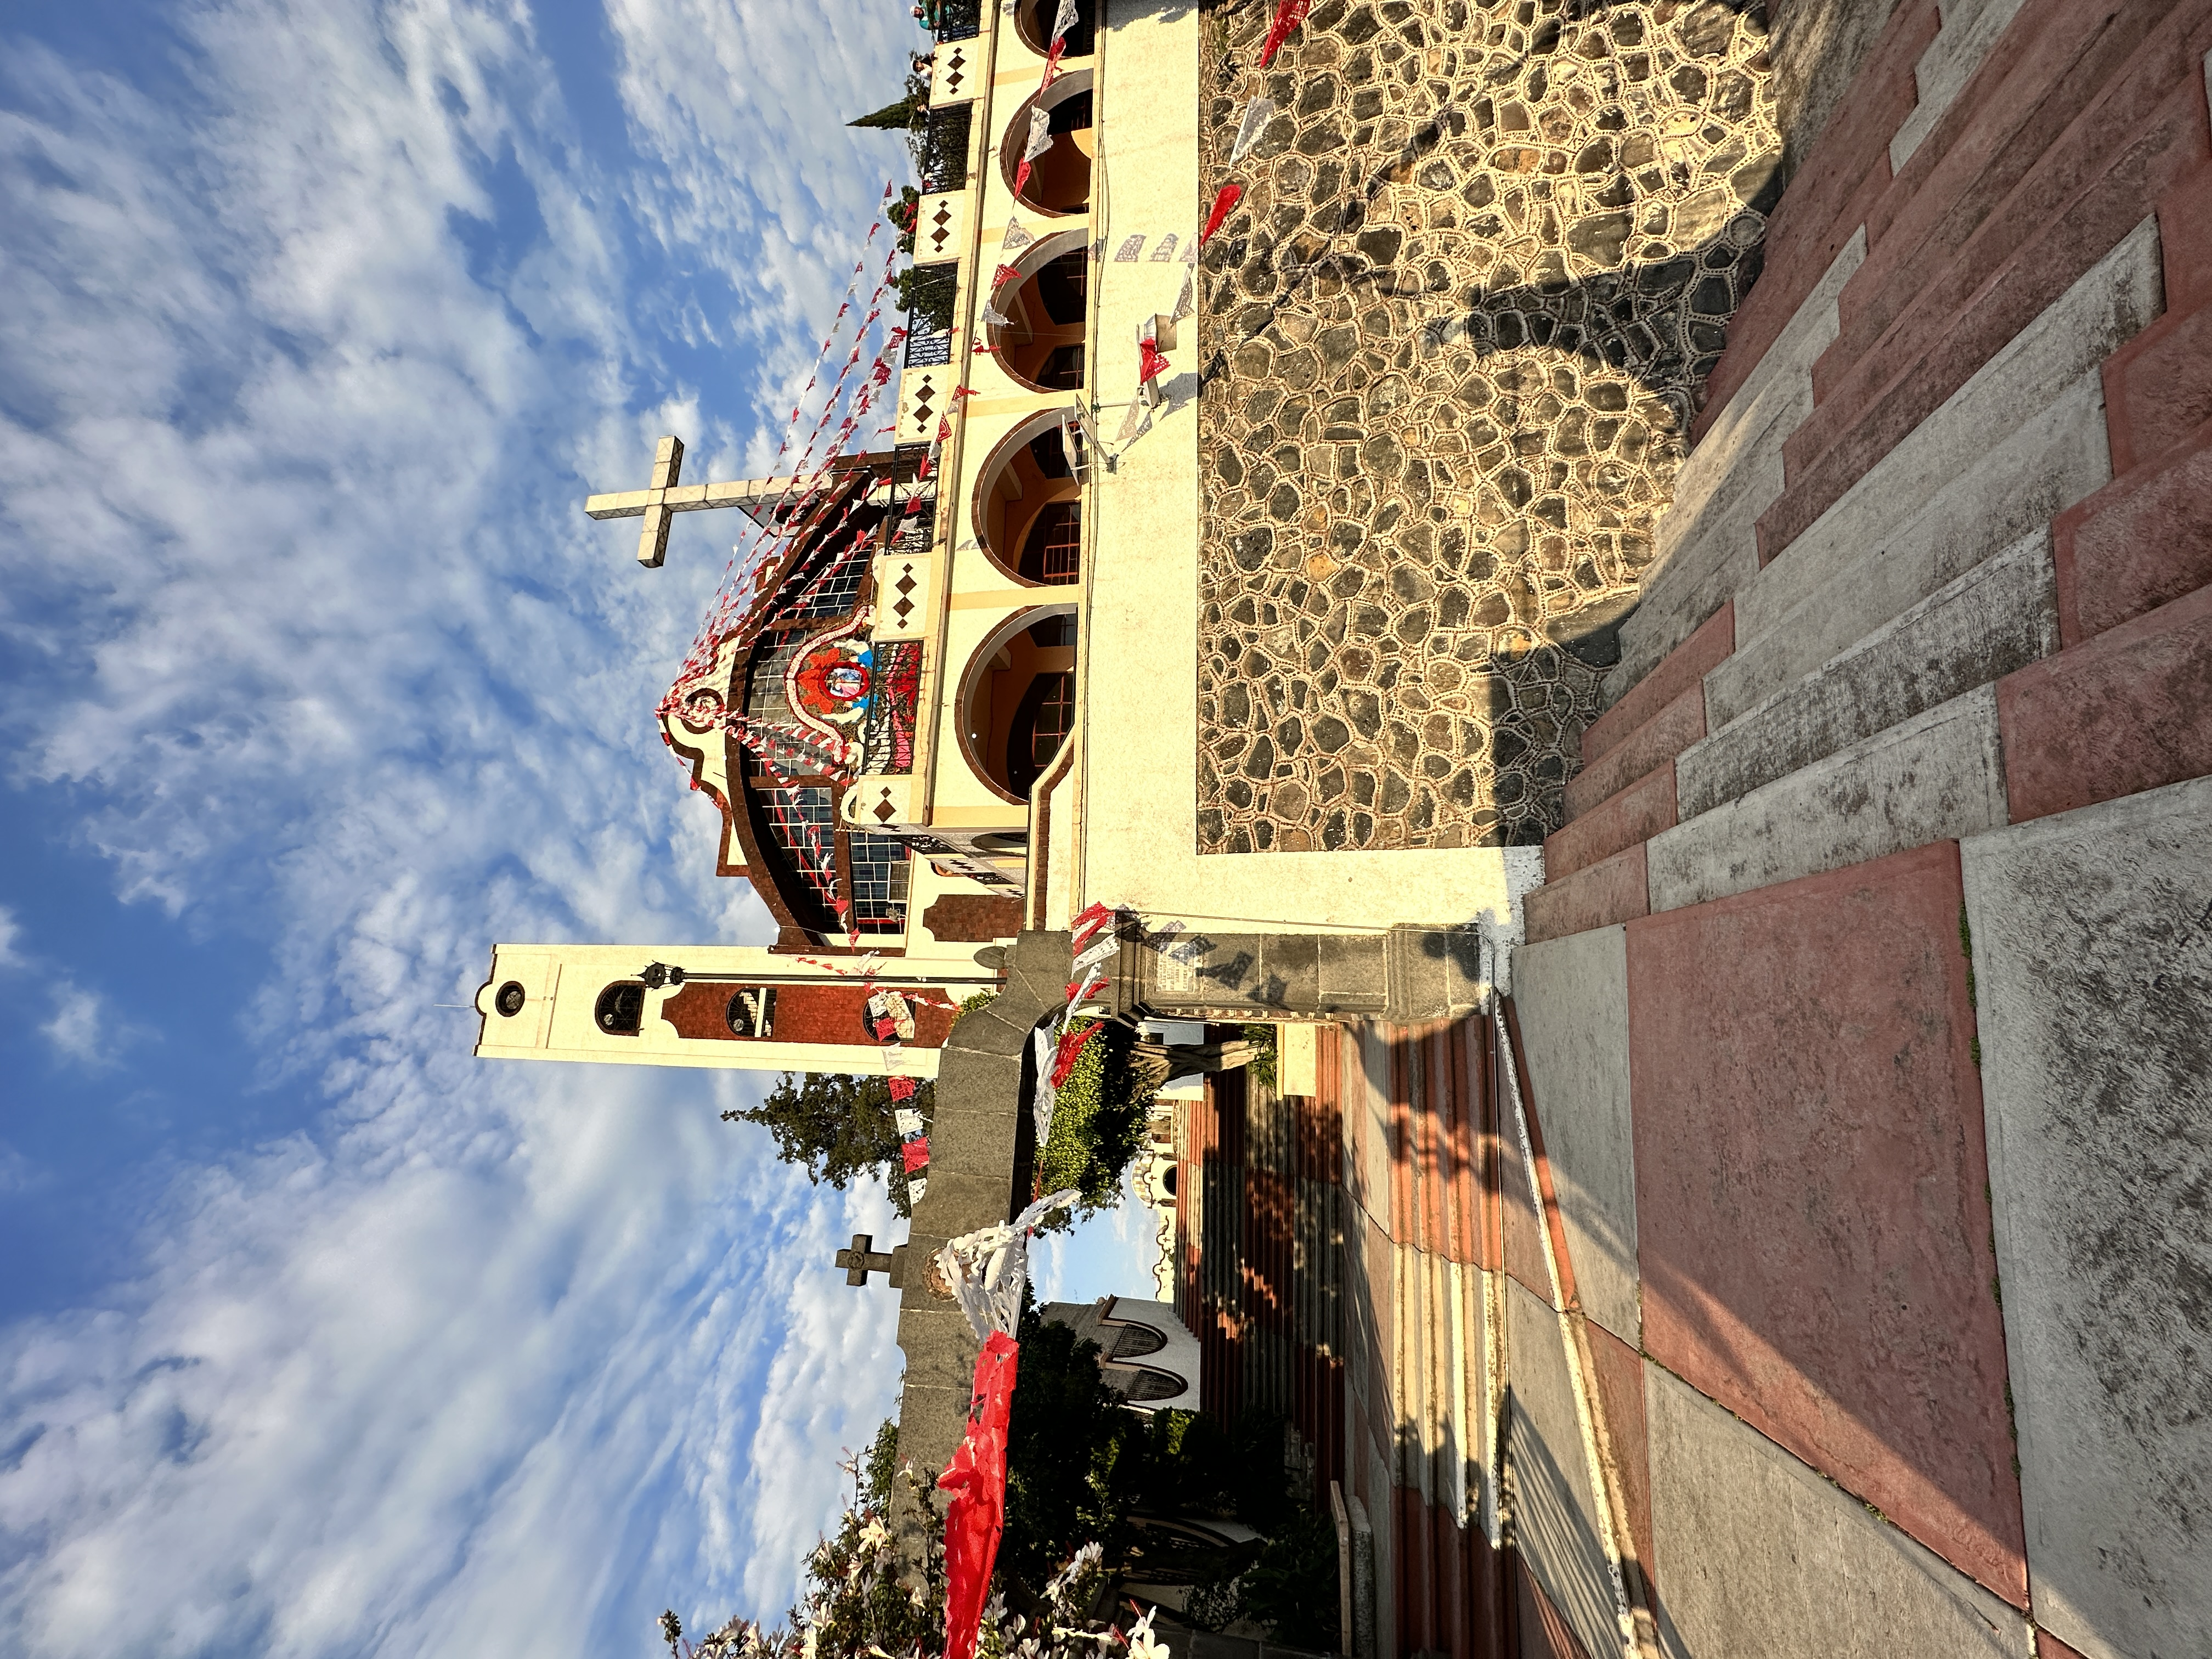
\includegraphics[width=\textwidth,height=7.2cm,keepaspectratio=false]{img/FotosActuales/TemploSrMisercordias/Templo2.JPEG}
        \caption{Vista angular del conjunto estructural y accesos peatonales.}
        \label{subfig:santuario-angular}
    \end{subfigure}
    
    \vspace{0.5cm} % Margen controlado entre filas de la cuadrícula
    
    % FILA 2: FOTOS INFERIORES (Detalles del entorno e integración urbana)
    \begin{subfigure}[b]{0.48\textwidth}
        \centering
        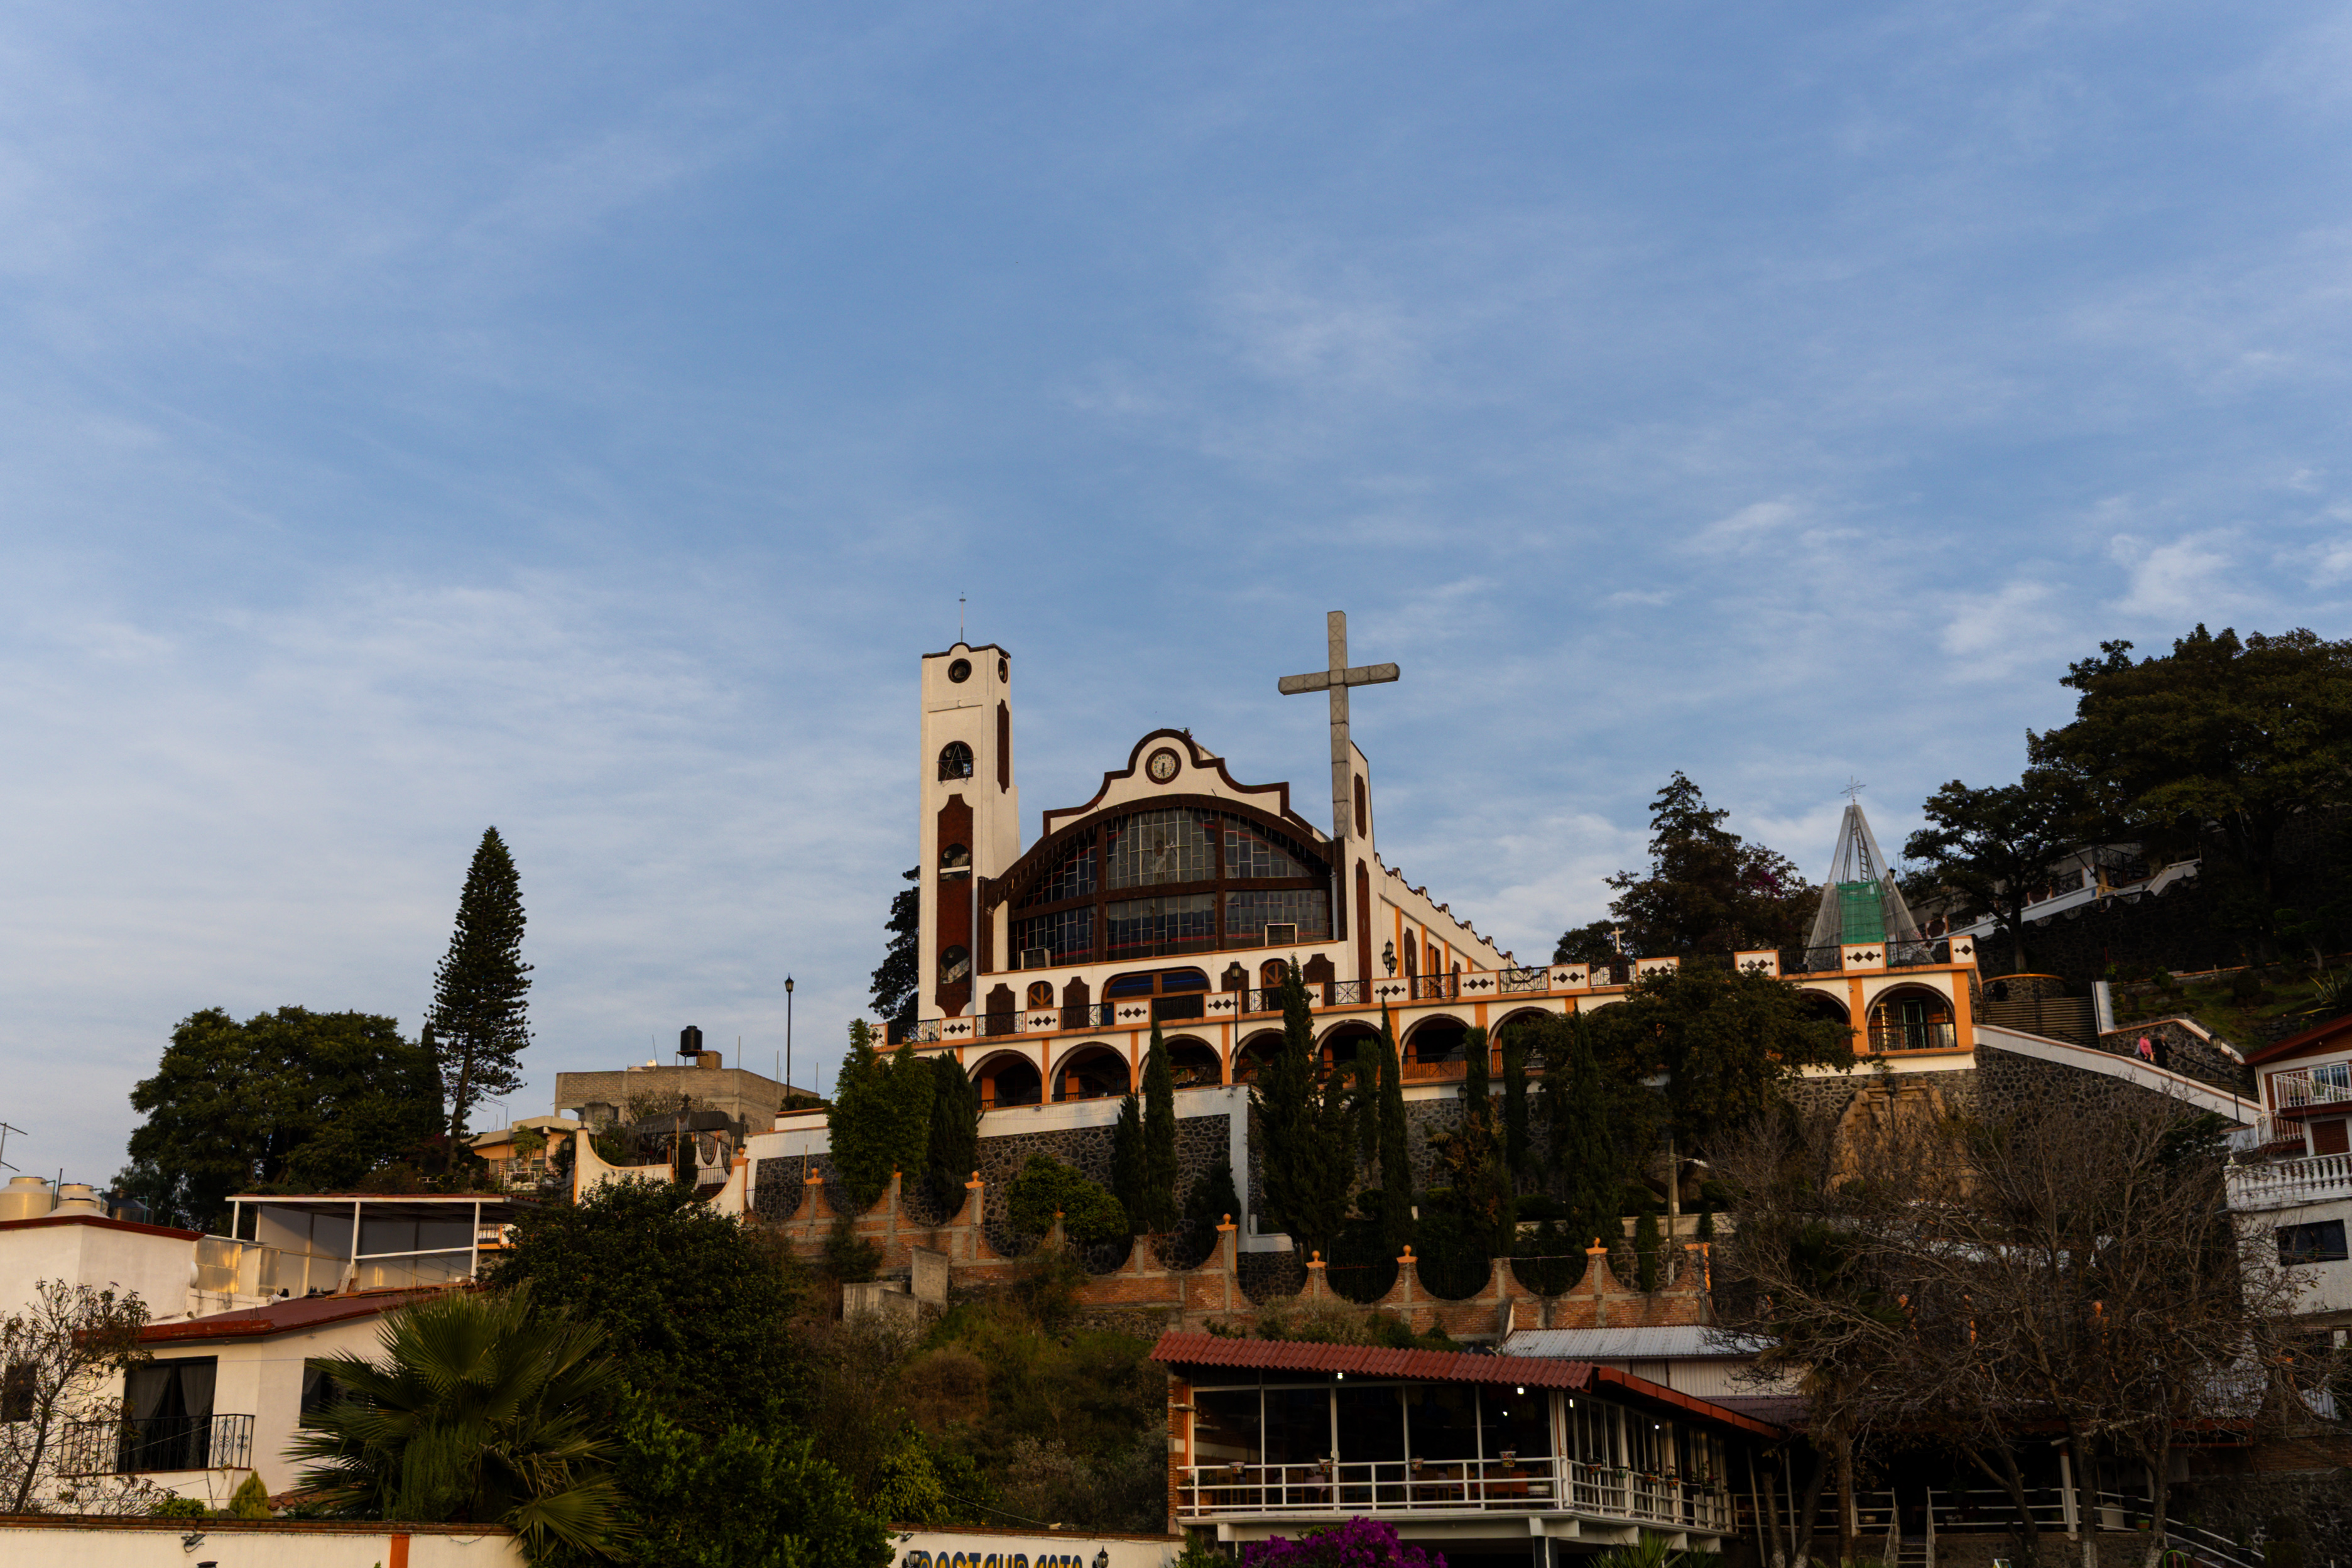
\includegraphics[width=\textwidth,height=7.2cm,keepaspectratio=false]{img/FotosActuales/TemploSrMisercordias/Templo3.JPEG}
        \caption{Articulación del volumen religioso con los niveles de la plaza.}
        \label{subfig:santuario-plaza}
    \end{subfigure}
    \hfill
    \begin{subfigure}[b]{0.48\textwidth}
        \centering
        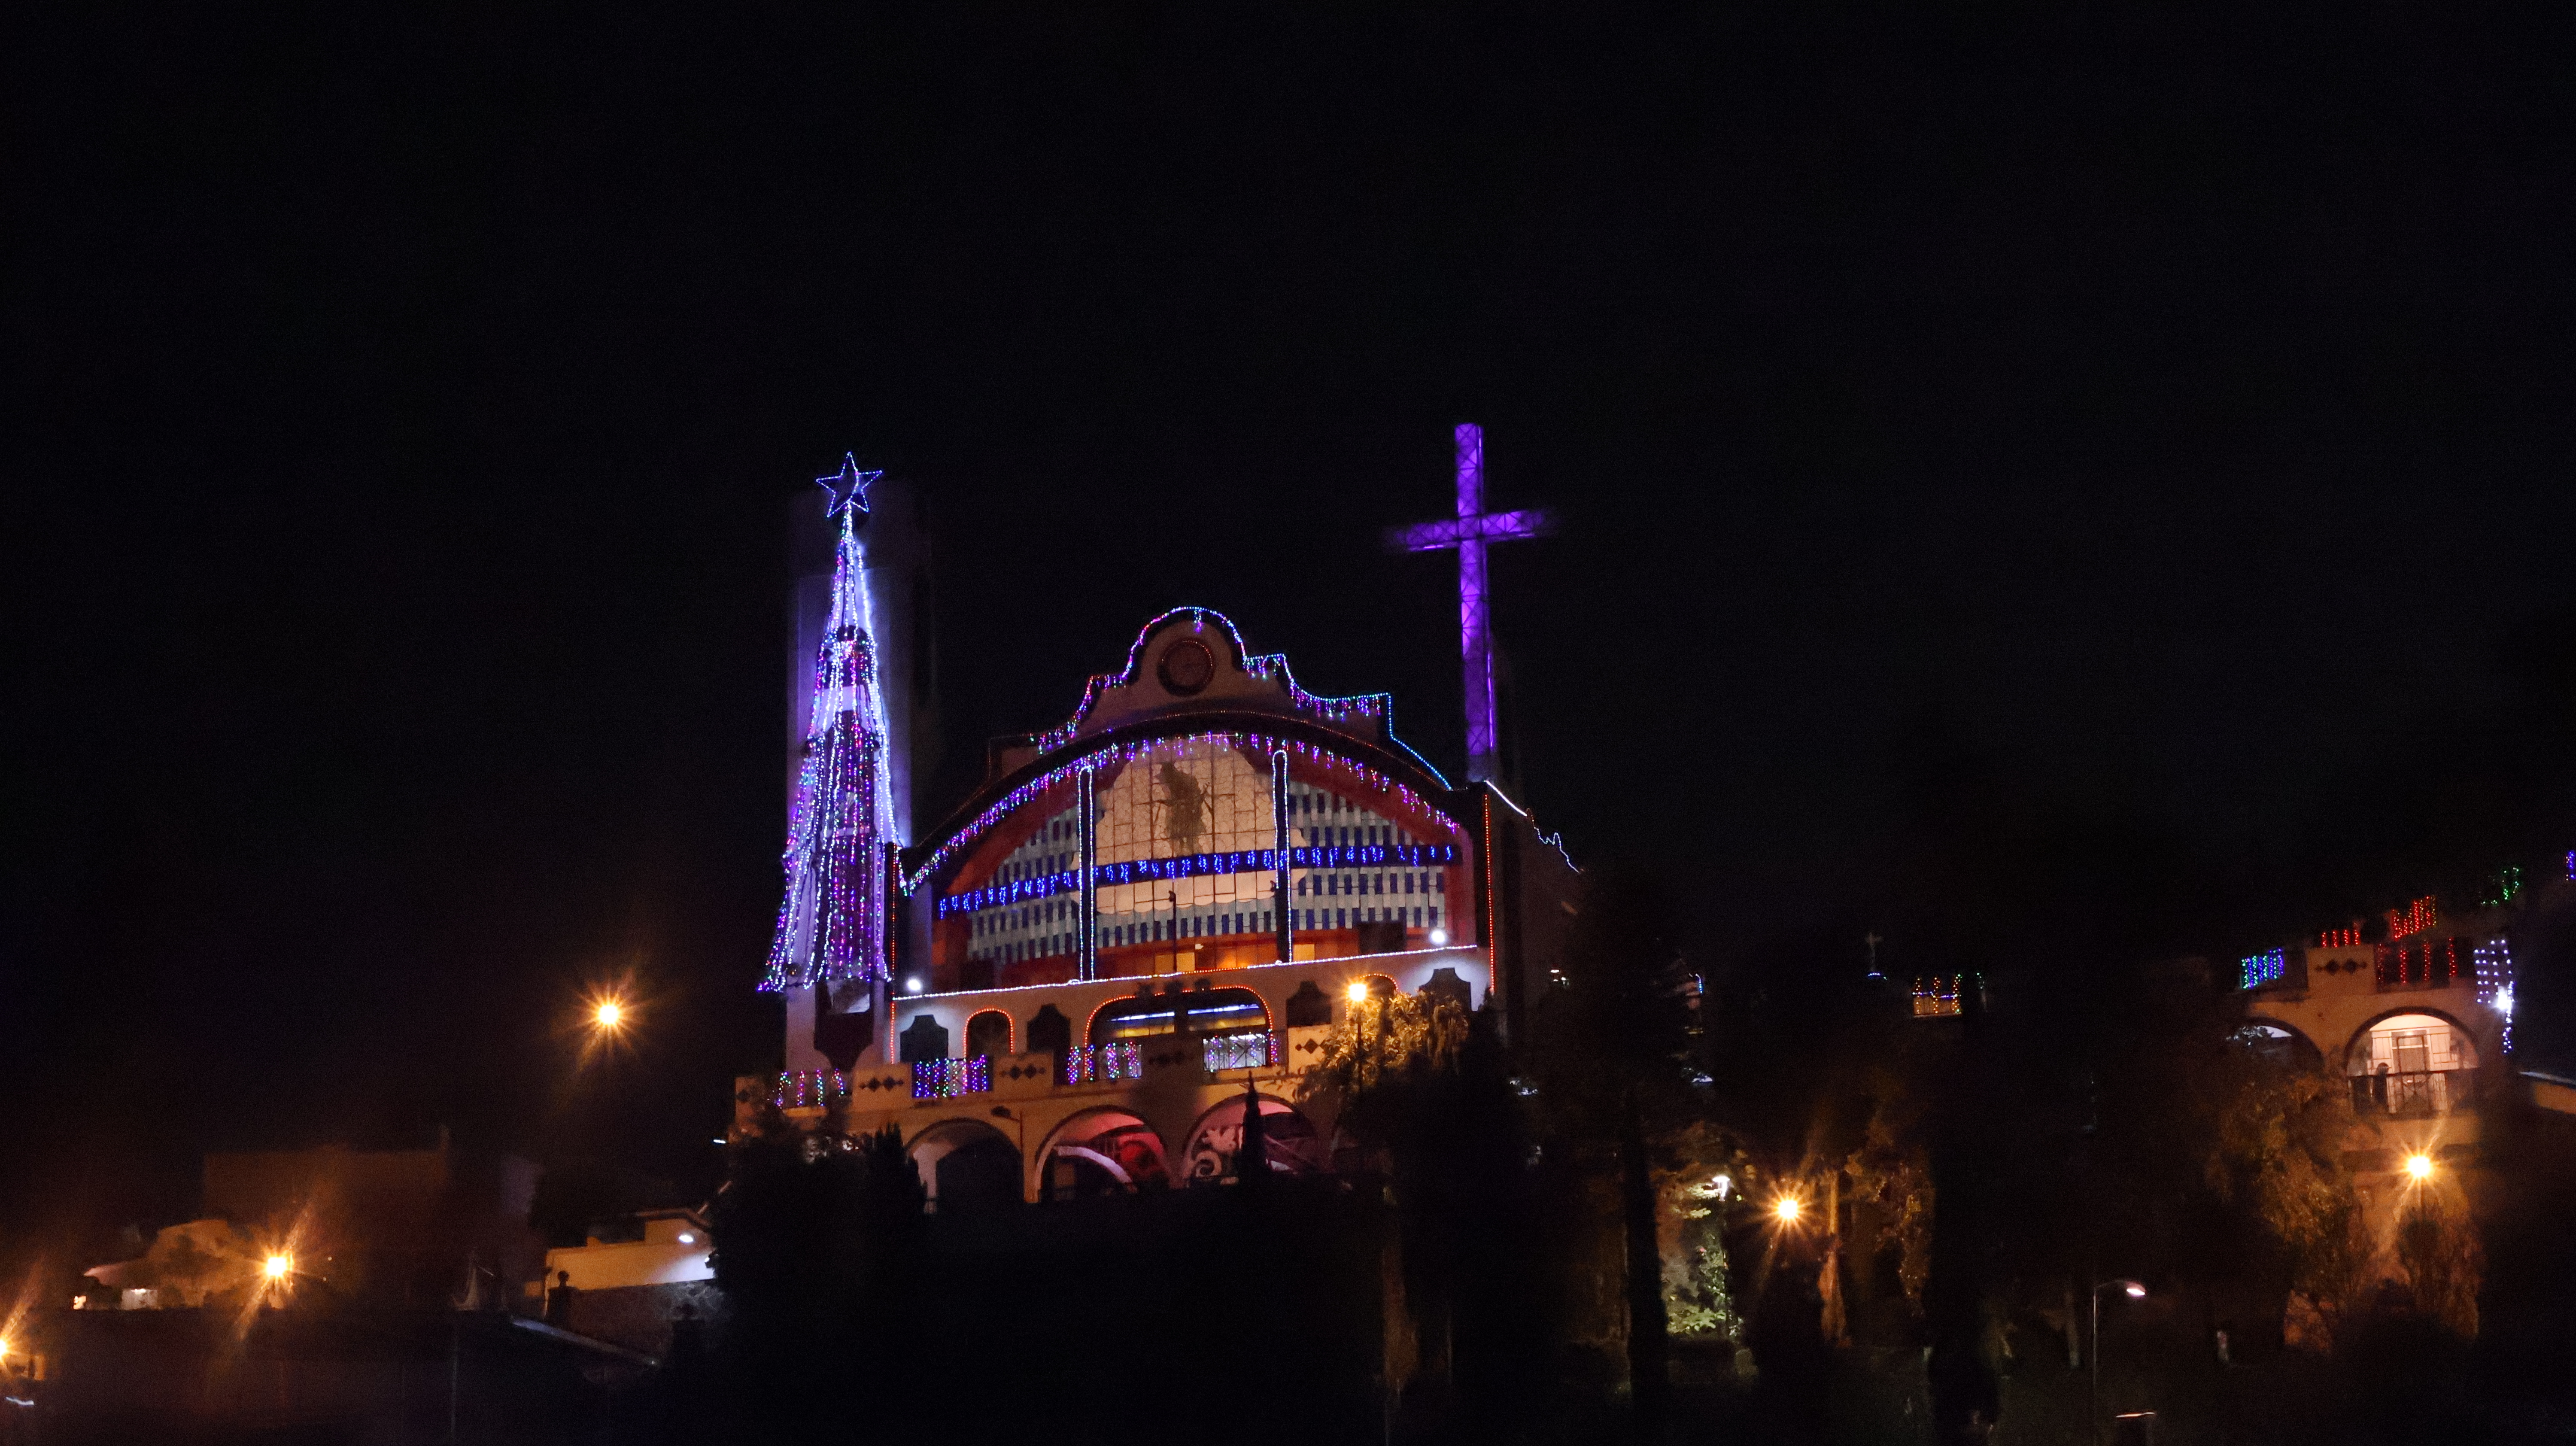
\includegraphics[width=\textwidth,height=7.2cm,keepaspectratio=false]{img/FotosActuales/TemploSrMisercordias/Templo4.JPEG}
        \caption{Relación de escala urbana y visuales desde el tejido circundante.}
        \label{subfig:santuario-entorno}
    \end{subfigure}
    
    \vspace{0.4cm}
    % Pie de figura con rigor metodológico de Plan Maestro
    \caption{Cuadrícula de análisis morfológico y constructivo del Santuario del Señor de las Misericordias. 
    \textbf{ID de Catálogo:} PRU-SPA-MOD-003. \textbf{Tipología:} Arquitectura religiosa moderna 
    (concluida a finales de la década de 1960). 
    \textbf{Ubicación:} Polígono 3, San Pedro Atocpan. 
    \textbf{Significancia:} Hito de soberanía comunal y cohesión social. 
    \textbf{Fuente y Autoría:} Fotografía de campo, obra original de la autoria del proyeccionista (Galigaribaldi).}
    \label{fig:cuadricula-santuario}
\end{figure}
\newpage